% This file was converted to LaTeX by Writer2LaTeX ver. 1.0.2
\documentclass{article}
\usepackage[utf8]{inputenc}
\usepackage[T1]{fontenc}
\usepackage[french]{babel}
\usepackage{amsmath}
\usepackage{amssymb,amsfonts,textcomp}
\usepackage{array}
\usepackage{hhline}
\usepackage{hyperref}
\hypersetup{colorlinks=true, linkcolor=blue, citecolor=blue, filecolor=blue, urlcolor=blue, pdftitle=, pdfauthor=Gilles Vuidel, pdfsubject=, pdfkeywords=}
\usepackage{graphicx}
\usepackage[top=2.501cm,bottom=2.501cm,left=2.501cm,right=2.501cm,nohead]{geometry}
\usepackage{float}
\usepackage{parskip}
\usepackage{multirow}
\usepackage{caption}
\makeatletter
\newcommand\arraybslash{\let\\\@arraycr}
\makeatother
% centering figures
\makeatletter
\g@addto@macro\@floatboxreset\centering
\makeatother
\setlength\tabcolsep{1mm}
\renewcommand\arraystretch{1.3}

% saut de page après une section
%\let\oldsection\section
%\renewcommand\section{\clearpage\oldsection}

% saut après itemize
\let\EndItemize\enditemize
\def\enditemize{\EndItemize\medskip}

\begin{document}
 \begin{titlepage}
	
	\centering
	
\includegraphics[scale=0.5]{img/logo.png}\\
	
	\bigskip
	\bigskip
	\bigskip	
	{\Huge
		\bfseries
		Graphab 2.0\\
		\bigskip
		Manuel d’utilisation\\
	}
	\bigskip
	\bigskip
	\bigskip
	\bigskip
	\bigskip
	
	{\Large		
		Céline Clauzel, Jean-Christophe Foltête, Xavier Girardet, Gilles Vuidel\\
		\bigskip
		12/05/2016\\
	}
	
\end{titlepage}

\setcounter{tocdepth}{2}
%\renewcommand\contentsname{}
\tableofcontents

\pagebreak

\section{Introduction}

\subsection{A propos de Graphab}

Le programme Graphab est un outil de modélisation des réseaux écologiques fondé sur les graphes paysagers. C'est un outil intégré composé de 4 modules : 
\begin{itemize}
	\item création de graphes à partir d'une carte de paysage avec identification des taches d'habitat et des liens (distance euclidienne ou chemin de moindre coût)
	\item calcul d'un grand nombre de métriques de connectivité
	\item intégration des métriques de connectivité dans un modèle de distribution d’espèce
	\item interface de géo-visualisation
\end{itemize}

La version 2.0 apporte plusieurs nouvelles fonctionnalités, dont :
\begin{itemize}
	\item l'ajout de taches,
	\item la création de méta-taches,
	\item le partitionnement de graphe,
	\item l'intégration du calcul de pente dans la création des liens,
	\item la théorie des circuits électriques.
\end{itemize}

\textbf{Attention, les projets ne sont pas compatibles entre les version 1.x et 2.x de Graphab !}

\subsubsection{Auteurs}
Le programme Graphab a été développé par Gilles Vuidel et Jean-Christophe Foltête au laboratoire \href{http://thema.univ-fcomte.fr}{ThéMA} (\href{http://www.univ-fcomte.fr}{Université de Franche-Comté} – \href{http://www.cnrs.fr}{CNRS}). Le développement du logiciel a été financé par le ministère de l'écologie, du développement durable, des transports et du logement dans le cadre du programme \href{http://www.ittecop.fr/}{ITTECOP}. Le logo de Graphab a été conçu par \href{http://www.gachwell.com/}{Gachwell}. 

\subsubsection{Conditions d’utilisation}
Le programme Graphab est disponible librement sous licence GPL. Les utilisateurs de Graphab sont invités à citer la référence \cite{2012_graphab_EMS} dans leurs travaux :

Foltête J.C., Clauzel C., Vuidel G., 2012. A software tool dedicated to the modelling of landscape networks. Environmental Modelling \& Software, 38: 316-327.


\subsection{Configuration requise}

Graphab fonctionne sur n'importe quel ordinateur supportant Java 7 ou supérieur (PC sous Linux, Windows, Mac...). Toutefois, lorsqu'il s'agit de données très volumineuses, la quantité de mémoire vive (RAM) de l’ordinateur peut limiter le nombre maximum de nœuds et de liens qui peuvent être traités en une seule fois avec Graphab. De plus, pour certaines métriques complexes, la puissance de votre processeur va déterminer la vitesse de leur calcul. Vous trouverez plus de détails à ce sujet dans la section \ref{limit} et dans \cite{2012_graphab_EMS}.

\subsection{Installation et lancement du programme}

Graphab est téléchargeable à cette adresse : \url{http://thema.univ-fcomte.fr/productions/graphab}.

\begin{itemize}
	\item Télécharger et installer Java 7 ou + (\href{http://www.java.com}{java.com}). Installer de préférence la version 64 bits de Java.
	\item Télécharger graphab-2.0.jar
	\item Lancer graphab-2.0.jar
\end{itemize}

Une fois graphab-2.0.jar lancé, le menu fichier donne accès à 4 rubriques : 
\begin{itemize}
	\item Fichier / Nouveau projet~: pour commencer la création d’un projet dans lequel toutes les données et résultats sont automatiquement enregistrés.
	\item Fichier / Ouvrir un projet : ouvre un projet déjà créé auparavant.
	\item Fichier / Préférences~: pour changer certains paramètres du programme : langue anglais/français ; quantité maximale de mémoire utilisable ; nombre de processeurs à utiliser. Il est recommandé d’adapter la quantité de mémoire et le nombre de processeurs aux capacités de l’ordinateur utilisé et aux traitements prévus (voir à ce sujet la section \nameref{limit}).  
	\item Fichier / Journal~: affiche le journal des évènements.
\end{itemize}

\section{Démarrer un projet Graphab}

La mise en place d’un nouveau projet Graphab s’effectue à partir du menu : Fichier / Nouveau projet. L’utilisateur doit renseigner plusieurs fenêtres successives : identification du projet, importation de la carte paysagère, création d’un jeu de liens. Un projet correspond à l’exploitation d’une seule carte paysagère initiale, mais il peut comporter plusieurs jeux de liens. Au terme de la phase de démarrage, le projet sera le support pour la création de multiples graphes et calculs de métriques de connectivité.

\subsection{Identification du projet}

Dans la première fenêtre, l’utilisateur doit nommer le projet et indiquer dans quel dossier celui-ci sera créé.

\begin{figure}[H]
	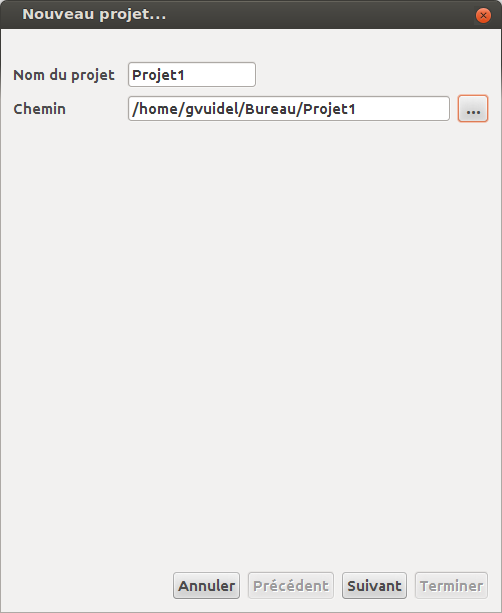
\includegraphics[scale=0.5]{img/manual-fr_img2.png} 
\end{figure}

\subsection{Importation de la carte du paysage et définition des nœuds}

La deuxième fenêtre concerne l’importation de la carte du paysage. Celle-ci doit être un fichier de type raster (*.tif, *.rst) dans lequel la valeur de chaque pixel correspond à une catégorie (occupation du sol ou autre type de classification).

\begin{figure}[H]
	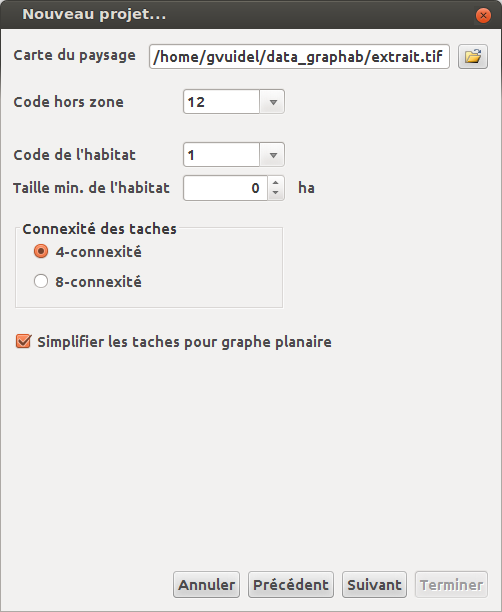
\includegraphics[scale=0.5]{img/manual-fr_img3.png} 
\end{figure}

S’il est en format *.tif, sans extension Geotiff, le fichier doit être associé à un fichier de géoréférencement (*.tfw) structuré comme suit :

\begin{table}[H]
\centering
\begin{tabular}{|m{3.552cm}|m{7.0800004cm}}
\hhline{-~}
Exemple & \\
\hhline{-~}
10.0 & Taille du pixel en X\\
0.0 & Rotation sur les lignes (0 pour les bonnes images)\\
0.0 & Rotation sur les colonnes (0 pour les bonnes images)\\
{}-10.0 & Taille du pixel en Y\\
821755.0 & Coordonnée en X du pixel haut gauche\\
2342995.0 & Coordonnée en Y du pixel haut gauche\\
\hhline{-~}
\end{tabular}
\end{table}

S’il est en format *.rst, le fichier doit être associé à un fichier de géoréférencement (*.rdc) suivant la structure proposée dans le logiciel Idrisi.

\textbf{Important ! L’unité du système de coordonnées de l’image doit être en mètre. Si ce n’est pas le cas, les unités de surface et de distance seront erronées. Il est possible de reprojeter l’image dans une projection métrique (Lambert93, UTM, …) à l’aide d’un SIG.}

Code hors zone : code des pixels correspondant à l’absence de valeurs dans le fichier raster.

Code de l’habitat : valeurs des pixels correspondant à l’habitat utilisé pour la définition des taches. Plusieurs valeurs peuvent être sélectionnées en maintenant la touche \verb|Ctrl|.

Taille min. de l’habitat : surface minimale en hectare pour qu’une tache d’habitat devienne un nœud du graphe.

Connexité des taches :
\begin{itemize}
	\item 4-connexité : une tache est constituée du pixel central et de ses 4 voisins~s’ils ont la même valeur ;
	\item 8-connexité : une tache est constituée du pixel central et de ses 8 voisins~s’ils ont la même valeur.
\end{itemize}

Simplifier les taches pour graphe planaire : cette option, lorsqu’elle est cochée, permet d’accélérer la création d’un graphe planaire, en simplifiant les limites des polygones des taches. Ce processus de simplification n’étant pas déterministe, la création de deux graphes planaires pour une même carte du paysage peut engendrer des limites de polygones légèrement différentes. Par conséquent, cette option ne doit pas être cochée dans le cas d’une comparaison de graphes planaires, par exemple quand on analyse les conséquences de changements d'occupation du sol sur la connectivité.

\subsection{Création d’un jeu de liens}
\label{linkset}
La troisième fenêtre concerne la création d’un jeu de liens, ce qui implique la sélection de plusieurs paramètres : topologie et pondération des liens. La création de ce jeu de liens constitue la dernière étape dans la mise en place initiale du projet. Cependant, il est possible de créer à tout moment de nouveaux jeux de liens dans le même projet, par le menu : Graphes / Créer un jeu de liens.

\begin{figure}[H]
	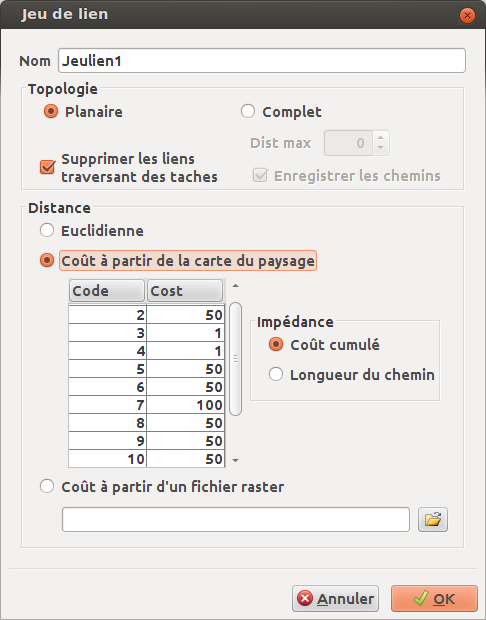
\includegraphics[scale=0.5]{img/manual-fr_img4.png} 
\end{figure}

\subsubsection{Topologie des liens}

Deux topologies sont disponibles :
\begin{itemize}
	\item planaire : seuls les liens formant un graphe planaire minimal sont pris en compte. Cette topologie est mise en place par l’intermédiaire de polygones de Voronoï autour de chaque tache d’habitat. Ces polygones sont définis à partir des bords des taches, en distance euclidienne.
	\item complet : tous les liens entre les taches sont potentiellement pris en compte.
\end{itemize}

Distance max : Cette option disponible pour la topologie complète permet de préciser un seuil de distance au-delà duquel les liens ne sont plus créés. Elle permet ainsi de limiter le nombre de liens créés et d’accélérer la création des liens en topologie complète.

Supprimer les liens traversant les taches : cette option, décochée par défaut, permet de ne pas créer de lien entre deux taches (A et C sur la figure suivante) passant par une tache intermédiaire (B). Ceci est recommandé pour le calcul de la métrique de centralité intermédiaire (BC) pour prendre en compte la fréquence avec laquelle chaque tache se trouve sur les plus courts chemins liant les paires de nœuds sur le graphe. A noter : cette option fournit une approximation de la distance intra-taches entre A et C. Si la case est décochée, un lien entre A et C passant par B sera créé représentant la distance complète réelle entre les deux taches. 

\begin{figure}[H]
	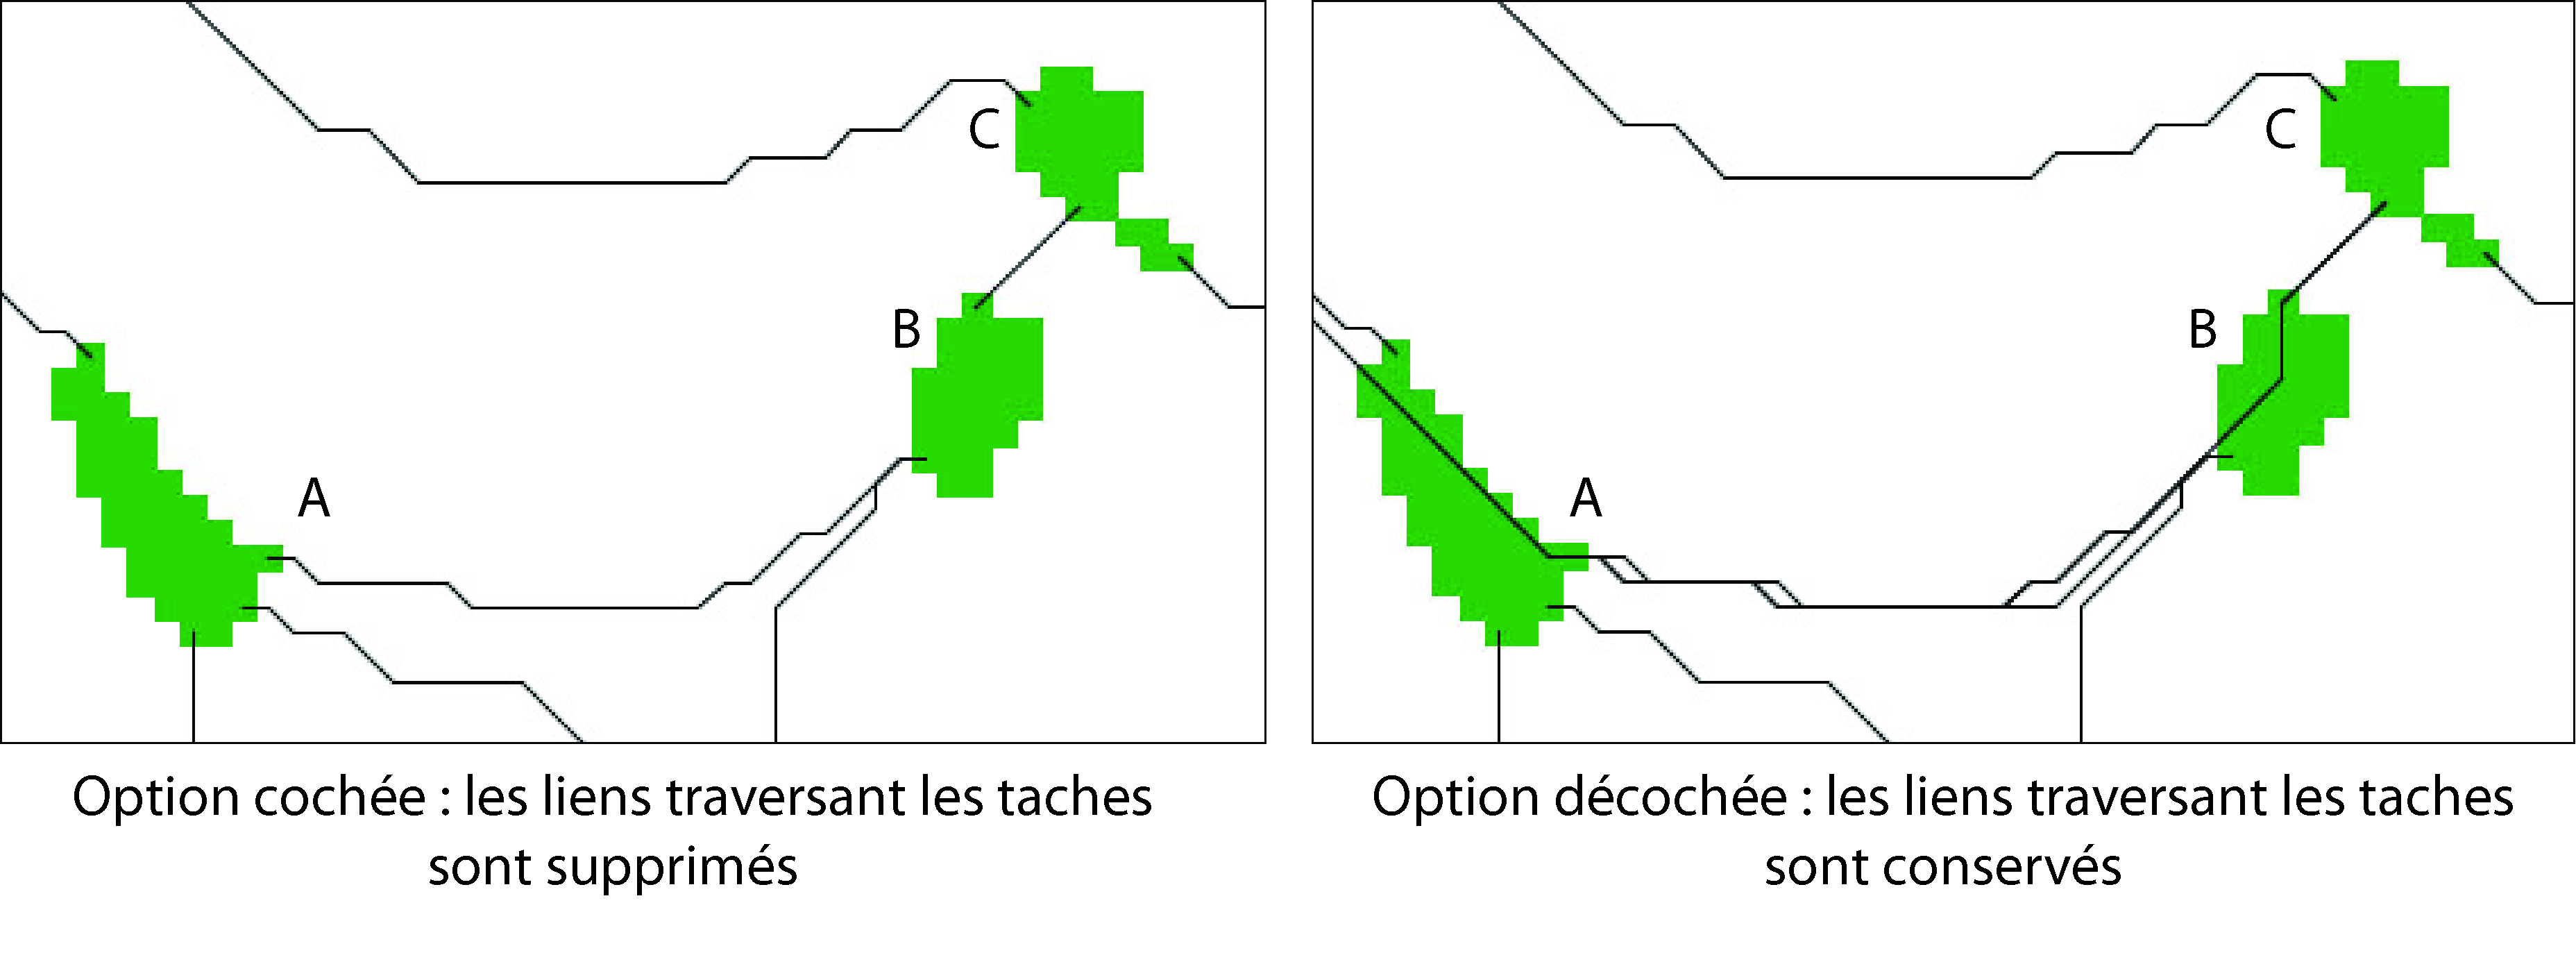
\includegraphics[scale=0.5]{img/manual-fr_img5.png} 
	\caption{Illustration de l’option «~Supprimer les liens traversant les taches~»}
\end{figure}
 

Enregistrer les chemins : 
\begin{itemize}
	\item si la case est cochée : les liens sont enregistrés sous forme de chemins représentant le tracé réel du lien entre deux taches. 
	\item si la case est décochée : les liens sont enregistrés sous forme topologique uniquement.  Dans ce cas, la visualisation des liens en vue réaliste n’est plus possible. Ceci est recommandé lorsque le graphe contient de nombreux liens (dans le cas d’un graphe complet non seuillé par exemple) afin de limiter l’utilisation de la mémoire. A noter : si les chemins ne sont pas enregistrés, il n’est pas possible d’inclure les distances intra-taches dans le calcul des métriques.
\end{itemize}


\subsubsection{Distance (ou impédance des liens)}

Les distances sont calculées de bord à bord entre les taches. Deux principaux types de distance sont possibles : distance euclidienne et distance de moindre coût.
\begin{itemize}
	\item Distance euclidienne :~les liens sont calculés en distance euclidienne (parcours à vol d’oiseau entre les taches), ce qui revient à considérer la matrice comme uniforme.
	\item Distance de moindre coût : les liens sont calculés en distance coût. L’hétérogénéité de la matrice est prise en compte en assignant des valeurs de résistance (ou friction) aux classes paysagères. L’utilisateur peut activer cette possibilité de deux façons :
	\begin{enumerate}
		\item soit en indiquant les coûts correspondant aux catégories de la carte du paysage dans le tableau ;
		\item soit à partir d’un fichier raster externe (format *.tif ou *.rst) contenant pour chaque pixel une valeur de résistance.
	\end{enumerate}
\end{itemize}

L’usage des distances de moindre coût donne accès à deux types d’impédance calculés à partir des mêmes chemins :
\begin{itemize}
	\item coût cumulé : l’impédance est égale à la somme des coûts de tous les pixels du chemin parcouru.
	\item longueur du chemin de moindre coût : l’impédance est égale à la longueur métrique du chemin parcouru.
\end{itemize}

Pour chaque lien créé, sa distance métrique et sa distance en unité de coût sont enregistrées et consultables dans les propriétés (cf. \nameref{properties}).

Les valeurs de résistance définies précédemment peuvent être pondérées par la pente \cite{2015_monkey}. Pour que la pente puisse être calculée, il faut tout d'abord charger un MNT à partir du menu Données | Importer un MNT. 

Le paramètre coef ($c$) permet d'ajuster l'importance de la pondération par la pente ($p$). Pour un pixel donné, la résistance résultante ($r_{final}$) est calculée comme suit :

$$r_{final} = r * (1 + c.p)$$

avec $p=\frac{h}{l}$ la pente exprimée par le rapport hauteur($h$) sur longueur ($l$).\\ $p=0$ pour une pente nulle et $p=1$ pour une pente de 100\% ($h=l$).

Pour $c=1$ la valeur de résistance est doublée avec une pente de 100\%.\\
Pour $c=10$ la valeur de résistance est doublée avec une pente de 10\%.

\section{Graphes}

\subsection{Création d'un graphe}
Un projet Graphab peut donner lieu à la création de plusieurs graphes. Chaque graphe étant construit à partir d’un jeu de lien, soit on utilise le jeu de lien défini lors de la mise en place initiale du projet, soit on définit un nouveau jeu de lien par le menu : Graphes / Créer un jeu de liens.

La création d’un graphe s’effectue par le menu : Graphe / Créer un graphe. 

\begin{figure}[H]
	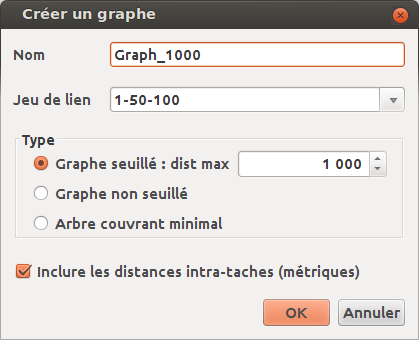
\includegraphics[scale=0.5]{img/manual-fr_img6.png} 
\end{figure}

Le graphe à créer doit tout d’abord être nommé.

L’utilisateur doit ensuite sélectionner un des jeux de liens créés précédemment (cf. \nameref{linkset}), puis choisir un type de graphe :
\begin{itemize}
	\item graphe seuillé : les liens retenus sont inférieurs ou égaux au seuil de distance choisi.
	\item graphe non seuillé : tous les liens sont créés~entre les taches quelle que soit leur distance.
	\item arbre couvrant minimal : graphe reliant toutes les taches dont le poids total des liens est minimal.
\end{itemize}

Option «~Inclure les distances intra-taches~» : si la case est cochée, le calcul des métriques à l’étape 3 tient compte des distances intra-taches (recommandé) ; dans le cas contraire, seules les distances inter-taches sont prises en compte.

Pour un graphe seuillé, l’unité de la distance de seuillage dépend du type de distance utilisé dans la création du jeu de liens. Si le jeu de lien a été créé en distance euclidienne, la distance de seuillage du graphe est exprimée en mètres. Si la création du jeu de lien a été réalisée en distance-coût, la distance de seuillage du graphe est exprimée en coûts cumulés. 

\begin{figure}[H]
	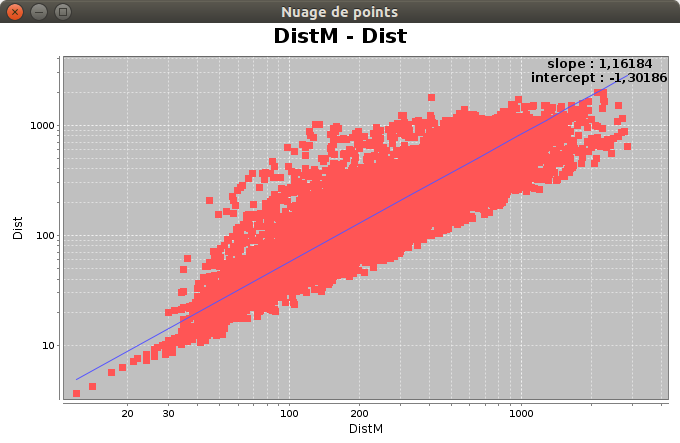
\includegraphics[scale=0.5]{img/manual-fr_img7.png} 
\end{figure}

Il est possible d’obtenir une approximation de la distance métrique (appelée DistM) exprimée en coûts cumulés (appelée Dist) en affichant le nuage de points en double logarithmique correspondant au jeu de lien utilisé, et en utilisant l'équation ci-dessous pour effectuer cette conversion :

$$Dist = e^{intercept + slope . log(DistM)}$$

L'estimation peut être réalisée directement dans le logiciel à partir du menu Conversion dist. présent dans le menu contextuel d'un jeu de lien (clic droit sur le jeu de lien).

Pour réaliser une analyse multiscalaire, il est souvent nécessaire de créer une série de graphes seuillés dont le seuil est défini de façon croissante. L’utilisateur peut créer manuellement cette série de graphes, mais si l’objectif est d’analyser le comportement d’une métrique de connectivité en fonction du seuil, il est préférable d’utiliser le menu : Métriques / Graphes par lot (cf. \ref{batch_graph}).

\subsection{Partitionnement de graphe}

Graphab implémente un algorithme de partitionnement de graphe qui maximise l'indice de modularité \cite{Newman2006}. La modularité est une mesure de la qualité d'un partitionnement des noeuds d'un graphe. Le principe sous-jacent est qu'un bon partitionnement d'un graphe implique un nombre de liens à l'intérieur des groupes important et un nombre de liens inter-groupes faible. Le calcul utilisé est basé sur l'algorithme glouton, suivi d'une optimisation locale \cite{Brandes2008}.

La modularité est calculée à partir d'un poids ($w_{ij}$) défini pour chaque lien du graphe :
$$w_{ij} = (a_i a_j)^\beta e^{-\alpha d_{ij}}$$
Les 2 paramètres $\beta$ et $\alpha$ permettent de définir respectivement l'importance de la capacité des taches ($a_i a_j$) et l'importance de la distance ($d_{ij}$) pour le poids du lien $w_{ij}$. Si $\alpha = \beta = 0$ alors les poids sont tous identiques : $w_{ij} = 1$.

Le partitionnement est accessible depuis le menu contextuel d'un graphe (clic droit sur le nom d'un graphe). La première fenêtre demande de renseigner les paramètres $\alpha$ et $\beta$. Le paramètre $\alpha$ n'est pas renseigné directement, il est déterminé à partir de deux autres paramètres : une distance $d$ et une probabilité $p$ (cf. \nameref{param_weight}). Pour définir $\alpha$ à 0, il faut mettre $p$ à 1. 

Après validation de cette fenêtre, le calcul se lance jusqu'à obtenir un partitionnement maximisant la modularité. Le résultat s'affiche sur une nouvelle couche du graphe. Deux autres fenêtres viennent compléter ce résultat. 

\begin{figure}[H]
	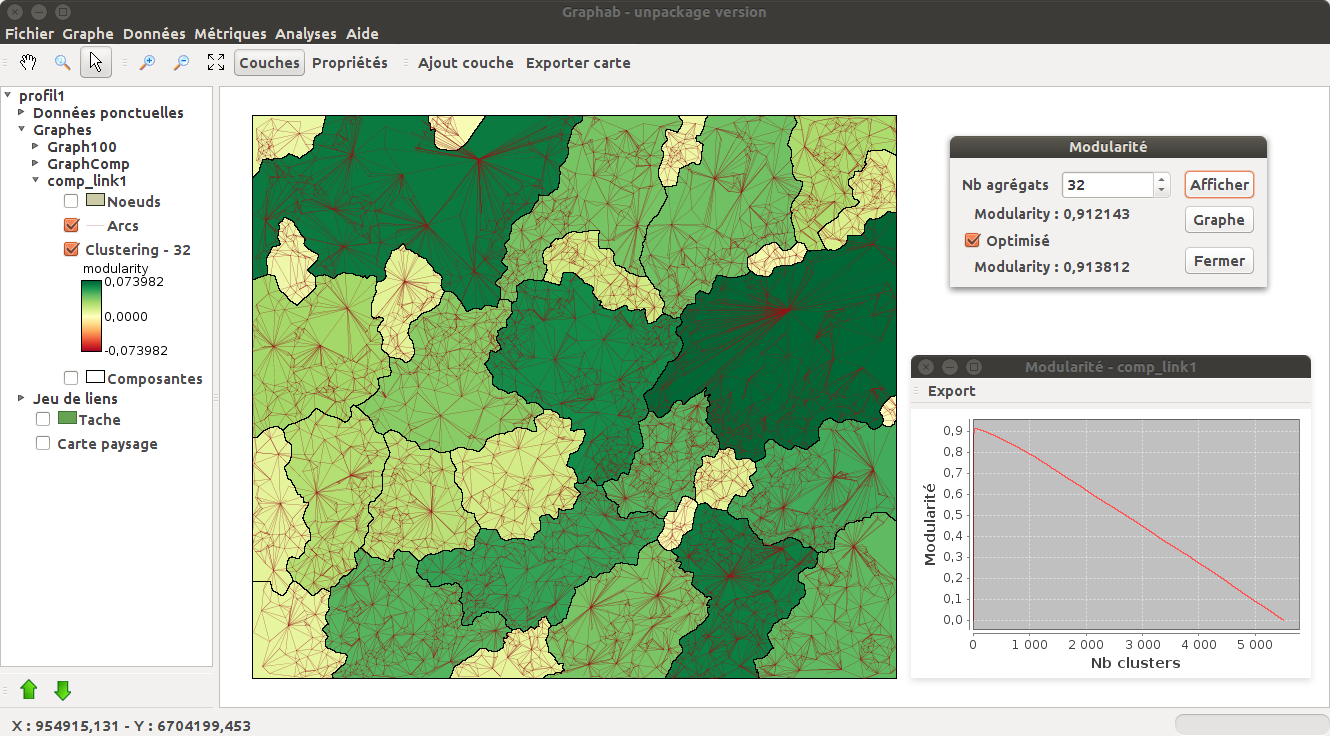
\includegraphics[scale=0.36]{img/manual-fr_cluster.png} 
\end{figure}

La nouvelle couche montre les groupes de la partition sous forme de polygones. Comme un groupe correspond à un ensemble de taches, il est représenté par un polygone agrégeant les polygones de Voronoï des taches affectées à celui-ci. 
La couleur d'un groupe correspond à sa valeur de modularité ; la modularité totale étant la somme des modularités de tous les groupes.

Une première fenêtre contient un graphique montrant l'évolution de la modularité en fonction du nombre de groupes (clusters). Dans la figure précédente, on voit que la modularité maximale est atteinte pour un nombre groupes relativement faible.

La deuxième fenêtre affiche le nombre de groupes (Nb agrégats) maximisant la modularité ainsi que la valeur de modularité. Plusieurs fonctionnalités sont disponibles sur cette fenêtre :

{}- le nombre de groupes peut être modifié pour visualiser des partitionnements sous optimaux. Le résultat peut être visualisé en cliquant sur le bouton "Afficher". Une nouvelle couche de partitionnement est ajouté au graphe.

{}- le bouton "Graphe" permet de créer un nouveau graphe ne contenant que les liens intra-groupes.

{}- la case à cocher "Optimisation" réalise une optimisation locale du partitionnement après l'algorithme glouton permettant d'améliorer sensiblement la valeur de modularité. Cette option est active par défaut.



\section{Capacité des taches}

La capacité d’une tache traduit sa «~qualité intrinsèque~», considérée comme un indicateur de son potentiel démographique. Ainsi une tache avec une forte capacité pourra accueillir une forte population et inversement. La capacité intervient directement dans le calcul de certaines métriques de connectivité «~de surface~» et «~pondérées~» (voir la section 5).

Par défaut (lors de la création initiale du projet), la capacité d’une tache est égale à sa superficie en m2. Cependant, il est possible de remplacer la superficie par n’importe quel autre indicateur de qualité. En effet, dans certains cas, la présence d’une espèce n’est pas liée à la superficie de la tache mais à la superficie d’autres types d’occupation du sol autour de la tache. Par exemple la présence d’amphibiens dans un étang de reproduction ne dépend souvent pas de la taille du plan d’eau mais de la superficie de l’habitat terrestre autour de ce plan d’eau.

Avec le menu Données / Définir la capacité des taches, il est possible de modifier la capacité de l'ensemble des taches du projet par deux méthodes.

\subsection{Capacité calculée comme une fonction du voisinage}

La première méthode est de définir la capacité des taches comme une fonction de la composition de leur voisinage et de procéder à ce calcul directement dans Graphab.

\begin{figure}[H]
	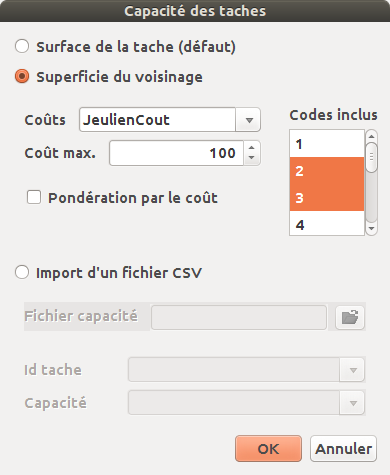
\includegraphics[scale=0.5]{img/manual-fr_img8.png} 
\end{figure}

L’utilisateur doit sélectionner plusieurs critères : type de distance, distance maximale, catégories paysagères.

Coûts : il s’agit de la métrique spatiale (euclidienne ou ensemble de coûts) correspondant à un des jeux de liens disponibles dans le projet. Il est à noter que l’usage des coûts dans cette procédure revient à définir un voisinage anisotropique autour des taches, ce qui peut différer fortement d’une fonction de type buffer. Pour des raisons de cohérence, il est conseillé d’utiliser le même type de distance que celui qui a permis de définir les liens du graphe. Dans le cas d’un jeu de lien créé avec une distance euclidienne, il faut choisir «~all cost = 1~».

Coût max. : Comme pour la distance de seuillage du graphe, l’unité de cette distance maximale de voisinage dépend du type de distance utilisé dans la création du jeu de liens (euclidien ou distance-coût).

Codes inclus : l’utilisateur peut choisir une ou plusieurs catégories paysagères, autre que la catégorie «~habitat~», ~à prendre en compte dans le calcul de la capacité. 

L’option «~pondération par la distance~» permet d’introduire une pondération en fonction de l’éloignement à la tache, par le biais d’une fonction exponentielle négative. De cette façon, les surfaces sélectionnées compteront plus si elles sont proches de la tache et inversement.

Les valeurs de capacité ainsi calculées remplacent les surfaces des taches pour tous les calculs qui suivront, mais il est possible de revenir à l’état initial par le menu : Données / Définir la capacité des taches et en cochant l'option Surface de la tache.

\subsection{Capacité définie à partir de données externes}

L'autre possibilité est d'ouvrir un tableau de données au format *.csv, décrivant toutes les taches du projet et contenant comme attribut les valeurs de capacité définies au préalable par l’utilisateur. Les identifiants du tableau importé doivent être ceux qui ont été définis lors de la création initiale du projet.

\begin{figure}[H]
	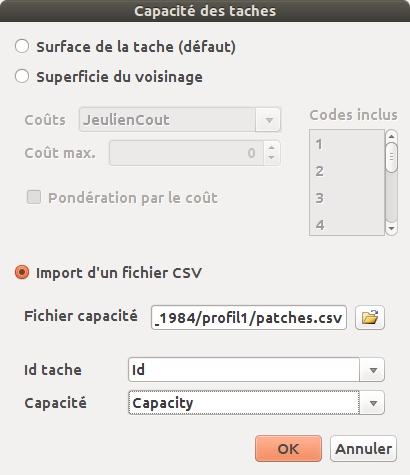
\includegraphics[scale=0.5]{img/manual-fr_img9.png} 
\end{figure}

Les valeurs de capacité du tableau importé remplacent les surfaces des taches pour tous les calculs qui suivront cette importation, mais il est possible de revenir à l’état initial en cochant l'option Surface de la tache.


\subsection{Suppression de taches}
Après avoir défini une capacité différente de la surface de la tache, il peut être intéressant de supprimer les taches dont la capacité est trop faible. L'entrée "Supprimer des taches" du menu Données, permet de créer un nouveau projet identique au projet actuel en supprimant les taches ayant une capacité inférieure à un seuil donné.

Après avoir renseigné la capacité minimale voulue, un nouveau projet est créé dans un sous répertoire du projet actuel et chargé à la fin du traitement.

\section{Calcul des métriques de connectivité}

\subsection{Famille de métriques et niveaux de calcul}

Chaque graphe créé dans un projet peut être utilisé pour calculer différentes métriques de connectivité, dont le détail de calcul et les références bibliographiques sont mentionnés en annexe. Ces calculs s’effectuent à plusieurs niveaux correspondant aux grandes entrées du menu Métriques (tableau \ref{metric_level}) :
\begin{itemize}
	\item Métriques /Métrique globale~: les métriques caractérisent le graphe entier.
	\item Métriques / Métrique par composante~: les métriques caractérisent la connectivité interne de chaque composante (ou sous-graphe).
	\item Métriques / Métrique locale~: les métriques caractérisent la connectivité de chaque élément du graphe, nœud ou lien.
	\item Métriques / Delta-métriques~: les métriques caractérisent également chaque élément du graphe, mais à partir d’un mode de calcul spécifique. En utilisant la méthode dite de la «~suppression~» (suppression de nœud ou suppression de lien), l’importance relative de chaque élément du graphe est évaluée en calculant le taux de variation que sa suppression occasionne sur une métrique globale. Le résultat d’une delta-métrique est donc local, mais en référence au niveau global.
\end{itemize}

Dans la fenêtre de dialogue qui s’ouvre suite au choix d’un de ces quatre modes de calcul, trois familles de métriques sont disponibles :
\begin{itemize}
	\item les métriques pondérées, qui sont fondées sur des critères de distance et de capacité des taches et qui nécessitent un paramétrage adapté à l’espèce de référence. Ces métriques nécessitent des calculs de chemin sur les graphes, par le biais de l’algorithme de Dijkstra. En choisissant ces métriques, l’utilisateur doit indiquer le réglage souhaité.
	\item les métriques de surface, qui sont fondées en priorité sur un critère de surface. Dans le cas où la capacité ne correspond pas à la surface des taches mais à un autre critère, ces métriques peuvent être calculées et elles s’expriment dans l’unité du critère considéré. 
	\item les métriques topologiques, qui sont issues de la théorie des graphes et qui ne nécessitent pas de paramétrage.
\end{itemize}


\begin{table}[H]

\begin{tabular}{|c|p{7cm}|l|c|c|c|c|}
\hline
\multirow{2}{*}{Famille} & \multirow{2}{*}{Métrique de connectivité} & \multirow{2}{*}{Code} & \multicolumn{3}{m{3cm}|}{\centering Niveau de calcul} & \multirow{2}{1.5cm}{Delta métriques}\\
\hhline{~~~---~}
 &  &  & Global & Comp. & Local & \\
\hline
\multirow{6}{2cm}{Métriques pondérées}
 & Flux & F & × & × & × & \\
 & Probabilité de connectivité & PC & × & × &  & ×\\
 & Probabilité de connectivité flux & FPC &  &  & × & \\
 & Fractions de delta Probabilité de connectivité & dPC &  &  &  & ×\\
 & Indice de centralité intermédiaire & BC &  &  & × & \\
 & Indice intégral de connectivité & IIC & × & × &  & ×\\
 & Flux circuit & CF &  &  & × & \\ 
\hline
\multirow{4}{2cm}{Métriques de surface}
 & Taille moyenne des composantes & MSC & × &  &  & \\
 & Taille de la plus grande composante & SLC & × &  &  & \\
 & Probabilité de coïncidence de classe & CCP & × &  &  & \\
 & Taille de composante attendue & ECS & × &  &  & \\
\hline
\multirow{9}{2cm}{Métriques topologiques}
 & Degré & Dg &  &  & × & \\
 & Coefficient de groupement & CC &  &  & × & \\
 & Centralité de proximité & CCe &  &  & × & \\
 & Excentricité & Ec &  &  & × & \\
 & Corrélation de connectivité & CCor &  &  & × & \\
 & Elément de coupure & Cut &  &  & × & \\
 & Nombre de composantes & NC & × &  &  & \\
 & Diamètre & GD & × & × &  & ×\\
 & Indice d’Harary & H & × & × &  & ×\\
\hline
\end{tabular}
\caption{Liste des métriques de connectivité et de leur niveau de calcul. Les codes sont indiqués suivant le nom anglais des métriques.}
\label{metric_level}
\end{table}

Quel que soit le niveau choisi, l’utilisateur doit d’abord indiquer le graphe sur lequel le calcul va s’appliquer, puis choisir la métrique de connectivité.

\subsection{Paramétrage des métriques pondérées}
\label{param_weight}

\begin{figure}[H]
	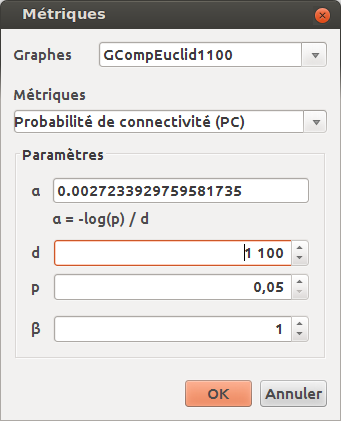
\includegraphics[scale=0.5]{img/manual-fr_img10.png} 
\end{figure}

\subsubsection{Paramètre alpha}

Plusieurs métriques intègrent dans leur calcul une pondération où les distances entre les taches sont converties en probabilité de déplacement. Ces métriques sont : F, FPC, PC, BC. La pondération est basée sur une fonction exponentielle de la forme :
\begin{equation*}
p={e}^{-\mathit{\alpha d}}
\end{equation*}
où p est la probabilité de déplacement entre deux taches, d la distance entre ces taches et $\alpha$ un paramètre contrôlant la vitesse avec laquelle la probabilité diminue quand la distance augmente. Comme la valeur du paramètre $\alpha$ n’est pas facile à déterminer, le logiciel propose de le calculer à partir des deux autres paramètres. L’utilisateur doit indiquer la distance correspondant à une certaine valeur de probabilité, par exemple :
\begin{itemize}
	\item la distance de dispersion maximale de l’espèce correspondant à une faible valeur de $p$ (0.05 ou 0.01).
	\item la distance de dispersion moyenne de l’espèce correspondant à une valeur médiane de $p$ (0. 5).
\end{itemize}
La valeur $\alpha $ est automatiquement obtenue à partir de la formule :
\begin{equation*}
\alpha =-\log \left(p\right)/{d}
\end{equation*}
Dans le cas d’un graphe seuillé, il est supposé que la distance $d$ utilisée dans ce paramétrage soit en cohérence avec celle qui a été utilisée pour le seuillage du graphe.

\subsubsection{Paramètre bêta}

Les mêmes métriques F, PC, FPC, BC sont contrôlées par le paramètre $\beta$. Ce paramètre est l’exposant appliqué à la capacité des taches. Il joue sur l’équilibre relatif entre le poids des distances et le poids des capacités des taches dans la pondération des métriques. En prenant l’exemple de la métrique F en calcul local, dont la forme générique est la suivante :
\begin{equation*}
F=\sum {{a}^{\beta }}{e}^{-\mathit{\alpha d}}
\end{equation*}

{}- une valeur de  $\beta =0$ signifie que la capacité des taches ne joue pas de rôle dans la pondération.

{}- une valeur de  $\beta =1$ signifie que la capacité des taches joue de façon linéaire dans cette pondération.

{}- une valeur de  $\beta =2$ signifie que la capacité des taches est portée à la puissance 2.

{}- une valeur de  $\beta =0.5$ signifie que la racine carrée de la capacité des taches intervient dans la pondération.

{}- une valeur de $\beta =-1$ signifie que la capacité des taches joue de façon inversement proportionnelle.

Au-delà de ces quelques exemples, toutes les valeurs de pondération sont possibles.

\subsection{Calcul des métriques par lot}

Chaque métrique compatible avec le niveau global peut être calculée en chaîne suivant la variation de l’échelle des distances. Cette variation peut concerner soit le seuillage du graphe (\ref{batch_graph}), soit le paramétrage des métriques elles-mêmes (\ref{batch_metric}). Le type de distance considéré pour le seuillage est celui qui a été défini pour le jeu de lien choisi, à savoir distance euclidienne, distance de moindre coût, chemin de moindre coût. 

\subsubsection{Graphes par lot}
\label{batch_graph}
Le menu Métriques / Graphes par lot permet de créer une série de graphes seuillés à partir d’un jeu de liens donné, et de calculer pour chacun une métrique de niveau global. Les seuils des graphes successifs sont définis de façon croissante, suivant deux modes :
\begin{itemize}
	\item distance : un intervalle de distance fixe est déterminé entre les graphes successifs. Les valeurs de la métrique sont donc calculées à des intervalles réguliers de distance.
	\item nombre de liens : un nombre de liens fixe est défini entre les graphes successifs. Ce nombre de liens est automatiquement transformé en distance utilisée pour seuiller le graphe. Ces distances seuil peuvent s’échelonner de façon irrégulière. 
\end{itemize}

\begin{figure}[H]
	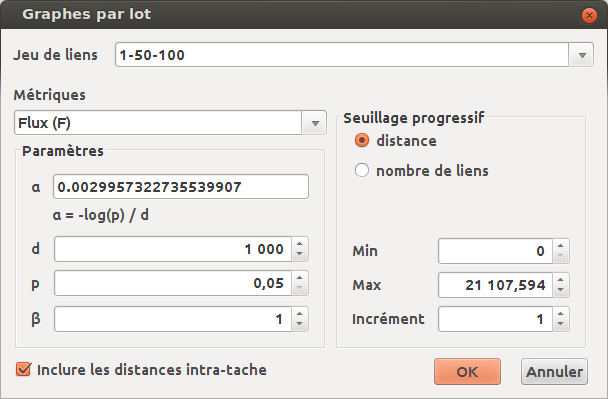
\includegraphics[scale=0.5]{img/manual-fr_img11.png} 
\end{figure}

Les graphes sont définis suivant trois critères donnés par l’utilisateur :
\begin{itemize}
	\item minimum : plus petit seuil, utilisé pour le premier graphe de la série. Par défaut, ce minimum est à 0, ce qui correspond à l’absence totale de liens.
	\item maximum : seuil maximal, utilisé pour le dernier graphe de la série. Par défaut, ce maximum correspond à la distance maximale, ou le nombre de lien, du jeu de lien sélectionné.
	\item incrément : valeur de distance ajoutée à chaque nouveau graphe.
\end{itemize}

Une fois le calcul terminé, le logiciel ouvre une nouvelle fenêtre dans laquelle la courbe de la métrique choisie est affichée en fonction du seuil de distance. Les valeurs de cette courbe peuvent être enregistrées par le bouton export, en sélectionnant le format texte.

\subsubsection{Paramètres par lot}
\label{batch_metric}
Le menu Métriques / Paramètres par lot permet de calculer en série des métriques à partir d’un graphe donné. Cette possibilité s’applique exclusivement aux métriques pondérées. Elle se subdivise en deux entrées : métriques locales ou globales.

\textbf{Paramètres par lot pour métriques locales}

Une métrique pondérée de niveau local est calculée en série suivant la variation d’un de ses paramètres. L’utilisateur doit choisir le graphe, la métrique et le paramètre à faire varier. La variation du calcul est déterminée par :
\begin{itemize}
	\item min : valeur minimale du paramètre
	\item max : valeur maximale du paramètre
	\item incrément : valeur d’intervalle entre deux calculs de la métrique
\end{itemize}

Une fois le calcul terminé, les taches (et dans certains cas les liens) du graphe sont caractérisées par une série de métriques supplémentaires.

\textbf{Paramètres par lot pour métriques globales}

Pour un graphe donné, une métrique pondérée de niveau global est calculée en série suivant la variation d’un de ses paramètres. Comme précédemment, cette variation est définie entre une valeur minimale (min), une valeur maximale (max) et un intervalle (incrément).

La procédure se termine par l’ouverture d’une nouvelle fenêtre dans laquelle la courbe de la métrique choisie est affichée en fonction du paramètre. 

Le tableau \ref{metric_poss} récapitule les possibilités de calcul des métriques.

\begin{table}[H]
\begin{tabular}{|c|m{5.162cm}|l|c|c|c|c|c|c|}
\hline
\multirow{2}{*}{Type} & \multirow{2}{*}{Métrique de connectivité} & \multirow{2}{*}{Code} & \multirow{2}{1.5cm}{\centering{Capacité des taches}} & \multirow{2}{1.5cm}{\centering{Distance intra-taches}} & \multicolumn{2}{m{1.8cm}|}{\centering Paramètres} & \multirow{2}{1.5cm}{\centering{Graphe par lot}} & \multirow{2}{1.55cm}{\centering{Paramètre par lot}}\\
\hhline{~~~~~--~~}
 & & & & & \multicolumn{1}{m{0.9cm}|}{\centering{$\alpha$}} & $\beta$ & & \\
\hline
\multirow{6}{2cm}{Métriques pondérées}
 & Flux & F & × & × & × & × & × & ×\\
 & Probabilité de connectivité & PC & × & × & × & × & × & ×\\
 & Probabilité de connectivité flux & FPC & × & × & × & × & × & \\
 & Fractions de delta Probabilité de connectivité & dPC & × & × & × & × &  & \\
 & Centralité intermédiaire & BC & × & × & × & × &  & ×\\
 & Indice Intégral de Connectivité & IIC & × &  &  &  & × & \\
 & Flux circuit & CF & × &  &  & × &  & ×\\
\hline
\multirow{4}{2cm}{Métriques de surface}
 & Taille moyenne des composantes & MSC & × &  &  &  & × & \\
 & Taille de la plus grande composante & SLC & × &  &  &  & × & \\
 & Probabilité de coïncidence de classe & CCP & × &  &  &  & × & \\
 & Taille de composante attendue & ECS & × &  &  &  & × & \\
\hline
\multirow{9}{2cm}{Métriques topologiques}
 & Degré & Dg &  &  &  &  &  & \\
 & Coefficient de groupement & CC &  &  &  &  &  & \\
 & Centralité de proximité & CCe &  & x &  &  &  & \\
 & Excentricité & Ec &  & x &  &  &  & \\
 & Corrélation de connectivité & CCor &  &  &  &  &  & \\
 & Nombre de composantes & NC &  &  &  &  & × & \\
 & Diamètre & GD &  & × &  &  & × & \\
 & Indice d’Harary & H &  &  &  &  & × & \\
\hline
\end{tabular}
\caption{Possibilités de calcul des métriques de connectivité.}
\label{metric_poss}
\end{table}


\subsection{Interpolation des métriques}

Le menu "Analyses / Interpoler une métrique" permet de générer des couches raster à partir des métriques locales calculées au niveau des taches. Cette transformation est fondée sur une interpolation spatiale spécifique, qui permet d’attribuer les valeurs de connectivité des taches à chaque cellule d’une grille, en utilisant une fonction de pondération décroissante à partir de la bordure des taches (poids de 1). Globalement, plus les cellules sont situées à l’écart du graphe, plus elles obtiennent des valeurs faibles de connectivité.

\begin{figure}[H]
	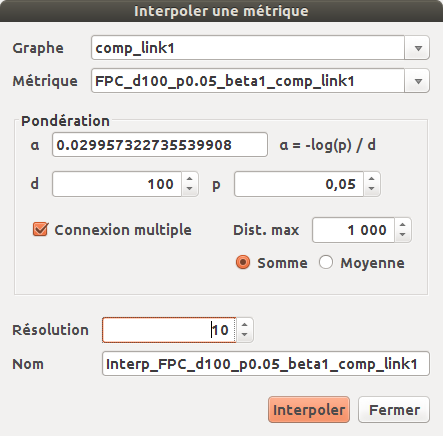
\includegraphics[scale=0.5]{img/manual-fr_img12.png} 
\end{figure}

La pondération est une fonction exponentielle négative de la forme  $p={e}^{-\mathit{\alpha d}}$ pour laquelle l’utilisateur doit choisir une distance (d) correspondant à une certaine probabilité (p) et le logiciel en déduit la valeur du paramètre $\alpha $. En principe, ce réglage est à rendre cohérent avec le choix du graphe de référence ou le choix des éventuelles métriques pondérées qui sont à mobiliser, en utilisant la même valeur de d.

L’option Connexion multiple permet de faire intervenir plusieurs taches dans le calcul des métriques au niveau des points. Le calcul est fondé sur une somme ou une moyenne pondérée des valeurs issues de toutes les taches comprises dans le voisinage des points, jusqu’à la Distance maximale indiquée.

Il est à noter que la distance considérée dans ces calculs dépend du graphe de référence. Si celui-ci est fondé sur une distance de moindre coût, l’interpolation spatiale utilise cette même distance et non une simple distance euclidienne.

L’interpolation des métriques est aussi utilisée automatiquement dans le calcul des modèles de distribution d’espèce (voir \nameref{sdm}).


\section{Ajout de taches}
La fonction "Ajout de taches" est accessible à partir du menu Analyses. Elle permet de tester un ensemble d’emplacements pour créer de nouvelles taches d’habitat en fonction du gain de connectivité qu’elles procurent. Le logiciel calcule d’abord la métrique globale sélectionnée, puis ajoute virtuellement une tache et les liens entre cette tache et les taches existantes (seulement si leur distance est inférieure au seuillage du graphe dans le cas d’un graphe seuillé) et recalcule la métrique globale. Une fois tous les emplacements testés, le logiciel valide l’emplacement qui procure le gain maximal de connectivité. La procédure est répétée jusqu’à l’ajout du nombre souhaité de nouvelles taches.

\begin{figure}[H]
	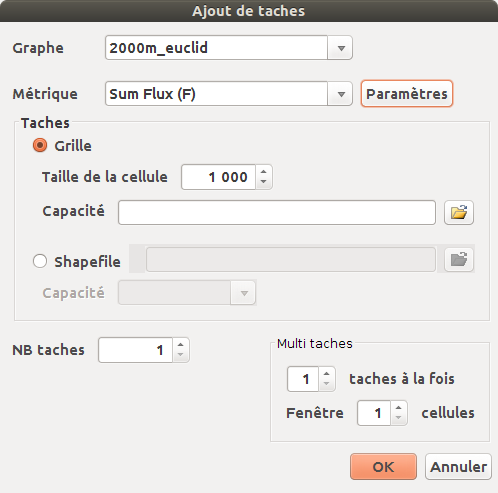
\includegraphics[scale=0.5]{img/manual-fr_addpatch.png} 
\end{figure}

Plusieurs paramètres sont à définir :
\begin{itemize}
	\item Graphe : le graphe utilisé pour le calcul de la métrique de connectivité et l’ajout de nouvelles taches. Le jeu de lien sous-jacent doit être en topologie complète.
	\item Métrique : la métrique globale que l’on cherche à maximiser ainsi que son paramétrage (bouton Paramètres)
	\item NB taches : nombre de taches (qui deviendront de nouveaux nœuds du graphe) que l’on souhaite ajouter.
\end{itemize}

La définition du jeu de taches à tester peut se faire de deux manières : 
\begin{itemize}
	\item En appliquant automatiquement une grille d’une certaine résolution (champs "taille de la cellule" à renseigner). Dans ce cas, le logiciel teste chaque centroïde de cellule en ajoutant virtuellement une nouvelle tache. Par défaut, tous les centroïdes ont une valeur de capacité identique (=1). Il est néanmoins possible d’importer une couche raster où chaque pixel de la matrice paysagère a une valeur de capacité propre.
	\item En important un shapefile de points ou de polygones. Il faut dans ce cas indiquer à quelle colonne de la table attributaire de ce shapefile correspond la capacité des taches.
\end{itemize}

Option "multi-taches" : cette option permet de tester l’ajout de plusieurs taches en simultané. Les taches supplémentaires sont recherchées dans une fenêtre de x cellules (paramètre à définir) autour de la première tache. 

A la fin du calcul, un répertoire nommé "addpatch\_nX-GraphX\_..." est créé et enregistré dans le répertoire du projet. Il contient :
\begin{itemize}
	\item un shapefile contenant les nœuds ajoutés. La table attributaire indique l’étape à laquelle a été validé chacun des nœuds et la valeur de la métrique globale correspondante.
	\item deux shapefiles contenant l’ensemble des liens du graphe, y compris ceux reliant les nouveaux noeuds, en version topologique ("topo\_links\_graphXXX") ou en version réaliste "links\_graphXX"
	\item un raster "landuse.tif" contenant l'occupation du sol modifiée
	\item un répertoire "détail" contenant pour chaque étape le shapefile des emplacements testés et la valeur de la métrique globale correspondant.
\end{itemize}

Références : 
\cite{2015_addpatch_rainette, 2014_LUP}

\section{Méta-taches}

À partir du menu Graphe, l'option "Créer un projet de méta-tache" permet de créer un nouveau projet où les noeuds du graphe correspondent à des ensembles de taches connectées à une certaine distance. Cette fonction permet de mieux prendre en compte l’emboîtement des échelles dans les processus écologiques et notamment le fait que la définition fonctionnelle d’une tache d’habitat varie selon l’échelle considérée (Theobald, 2006 ; Zetterberg et al., 2010).

\begin{figure}[H]
	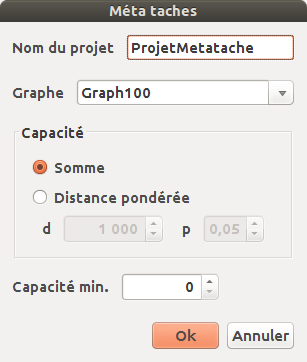
\includegraphics[scale=0.5]{img/manual-fr_metapatch.png} 
\end{figure}

Pour utiliser cette fonction, il est nécessaire de créer un projet initial et un graphe seuillé à la distance souhaitée (par exemple à la distance quotidienne). Chaque composante de ce graphe seuillé correspondra à une méta-tache. Celle-ci est donc constituée de l’ensemble des taches d’habitat connectées entre elles.

La capacité des méta-taches est définie par défaut comme la somme de la capacité des taches composant la méta-tache. L'autre option "Distance pondérée" permet de tenir compte de l'éloignement des taches entre elles. Pour cette option, il faut définir le paramètre $\alpha$ en donnant une distance $d$ et une probabilité $p$ associée (cf. \nameref{param_weight}). La capacité résultante ($C$) d'une méta-tache s'écrit : 

$$C = \frac{1}{n}\sum_{i}^n\sum_{j}^n c_j e^{-\alpha d_{ij}}$$ 

L’option "capacité minimale" permet de ne garder pour le nouveau projet que les méta-taches qui ont une capacité supérieure ou égale au seuil défini.

Le nouveau projet est enregistré dans un sous répertoire du projet initial et est chargé automatiquement à la fin du traitement.

Références : \cite{2015_monkey}


\section{Liens entre graphes et données ponctuelles}

Le corps principal du logiciel est la mise en place des graphes et le calcul de métriques de connectivité, mais il est souvent très utile de relier ces éléments à des données externes. Le logiciel permet de faire interagir les données issues des graphes avec un jeu de données de points.

\subsection{Import de données ponctuelles}

Des données ponctuelles peuvent être importées par le menu : Données / Importer des données ponctuelles. Ces données peuvent contenir plusieurs attributs, mais seuls les attributs binaires (présence/absence) seront pris en compte dans certaines procédures (voir Modèles de distribution d’espèce au 6.3).

\begin{figure}[H]
	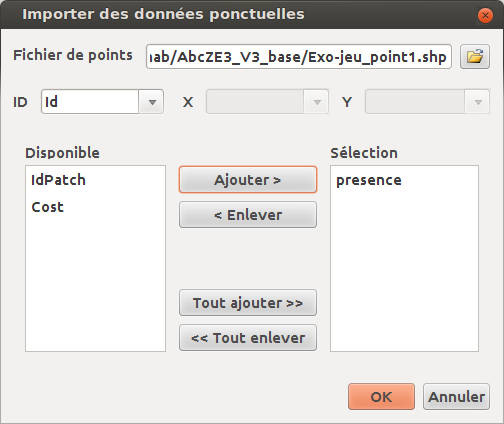
\includegraphics[scale=0.5]{img/manual-fr_img13.png} 
\end{figure}

Le fichier importé peut être soit sous forme de couche vectorielle au format shapefile (*.shp), soit sous forme de tableau (*.csv). Dans le second cas, il faut indiquer les colonnes du tableau qui correspondent aux identifiants et aux coordonnées en X et en Y des points. Les attributs à prendre en compte doivent être sélectionnés à partir de la liste des attributs disponibles.

Si les données ponctuelles ne contiennent pas d’attribut d’absence, elles ne peuvent pas être utilisées dans des modèles de distribution d’espèce. Si l’utilisateur envisage de mettre en place un modèle de distribution d’espèce, l’utilisateur doit créer un jeu de données de pseudo-absence avec Données / Générer des points aléatoires.

\subsection{Matrices de distance inter-points}

Les données ponctuelles importées dans Graphab peuvent être à l’origine du calcul de matrices de distance inter-points par le menu Matrice de distance du menu contextuel d'un jeu de points (clic droit sur le nom d’un jeu de points).

\begin{figure}[H]
	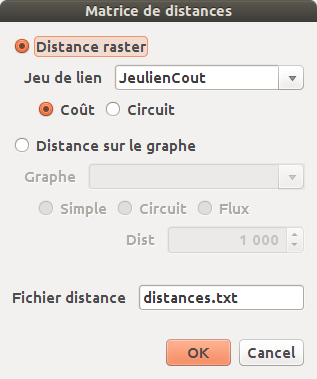
\includegraphics[scale=0.5]{img/manual-fr_img13b.png} 
\end{figure}

Les distances peuvent être calculées de 2 manières : directement sur le raster ou bien à travers un graphe.

\subsubsection{Distance raster}
En mode raster, les distances sont calculées en fonction d'un jeu de lien de référence. Ce jeu de lien ne peut pas être en distance euclidienne.

Selon le jeu de lien choisi, il peut s’agir de la distance coût cumulée ou de la longueur du chemin de moindre coût. Dans les deux cas, le calcul intègre les coûts associés aux catégories de la carte de paysage, tels qu’ils ont été définis dans le jeu de liens. Le résultat est une matrice de distance indépendante du graphe ; cette matrice correspond au calcul offert par les Systèmes d’Information Géographique.

L'option Circuit permet de calculer la "distance de résistance" entre chaque point, c'est-à-dire la résistance équivalente d'un réseau de résistances électriques au lieu du calcul du chemin le plus court. Cette méthode permet de tenir compte de l'ensemble des chemins possibles et non pas uniquement du plus court (cf. \cite{McRae2008}).


\subsubsection{Distance sur le graphe}

En mode graphe, les distances sont calculées en fonction du graphe sélectionné. Ce graphe doit être basé sur le jeu de lien utilisé à l'import du jeu de point.

\begin{itemize}
	\item Simple : distance calculée suivant le plus court chemin sur le graphe de référence. Le type de distance correspond à celui qui a été utilisé pour la définition du jeu de lien qui a servi à définir le graphe de référence. Aux deux extrémités du chemin considéré, le calcul intègre la distance entre chaque point et la tache la plus proche. Suivant le choix qui a été fait au moment de la création du graphe, le calcul intègre éventuellement les distances intra-taches.	
	\item Circuit : calcule la "distance de résistance" entre les taches les plus proches de chaque point. Le graphe est vu comme un réseau électrique où chaque lien du graphe représente une résistance. Cette option permet de tenir compte de l'ensemble des chemins possibles et non pas uniquement du plus court.
\end{itemize}

\subsection{Générer des points aléatoires}

Le menu Données / Générer des points aléatoires permet de créer un ensemble de points de pseudo-absence en s’appuyant sur un ensemble de points de présence.

\begin{figure}[H]
	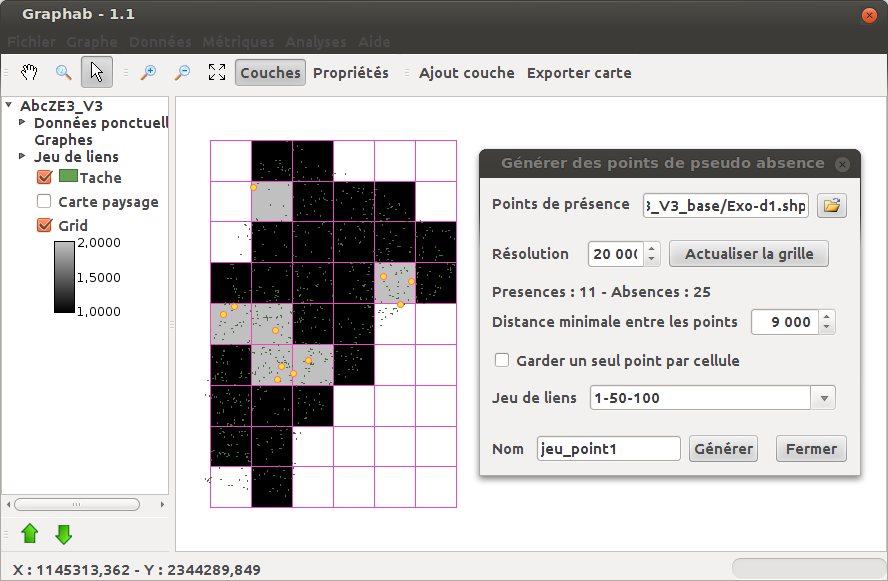
\includegraphics[scale=0.5]{img/manual-fr_img14.png} 
\end{figure}

L’utilisateur doit charger un fichier de points de présence et indiquer le nom du jeu de points de présence / absence à créer.

Plusieurs paramètres sont à définir pour effectuer un tirage aléatoire des points d’absence :

{}- Résolution de la grille (en mètres) pour définir la taille des cellules dans lesquelles seront éventuellement tirés des points d’absence. Le bouton «~actualiser la grille~» permet d’afficher la grille selon la résolution choisie

{}- Distance minimale entre les points (en mètres) : cette fonction permet d’atténuer les effets d’autocorrélation spatiale en indiquant une distance minimale à respecter entre les points d’absence générés et entre ces points et les points de présence. 

{}- Type de distance : l’unité de la distance minimale entre les points dépend du type de distance utilisé dans le jeu de liens sélectionné.

{}- Garder un point par cellule : cette option permet de ne garder qu’un point de présence dans chaque cellule pour atténuer les effets d’autocorrélation spatiale.

\subsection{Modèle de distribution d’espèce}
\label{sdm}

Si un jeu de points de présence / absence a été défini, le logiciel permet d’utiliser les métriques de connectivité calculées à partir d’un graphe comme variables prédictives dans un modèle de distribution d’espèce, suivant le menu Analyse / Estimation du modèle. Cette modélisation est possible même si les points ne sont pas situés dans les taches d’habitat, par le biais d’une extrapolation spatiale des valeurs des métriques. Le modèle est une régression logistique fondé sur la minimisation du critère AIC.

\begin{figure}[H]
	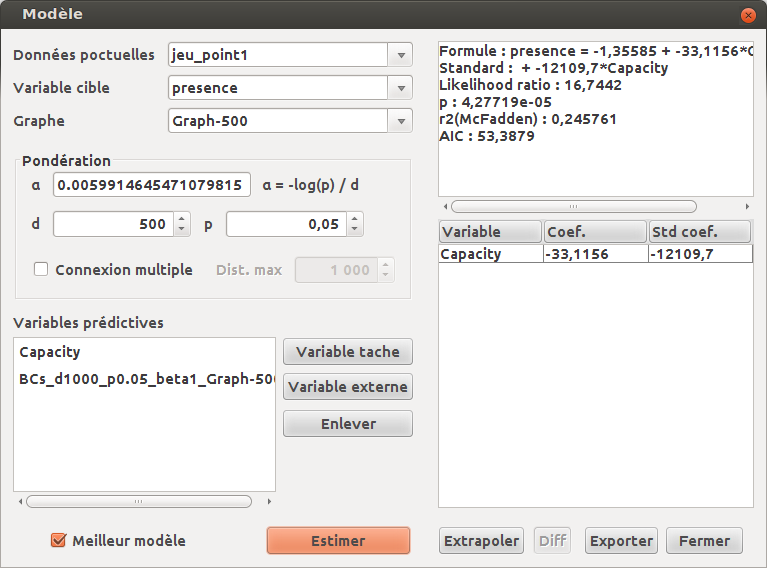
\includegraphics[scale=0.5]{img/manual-fr_img15.png} 
\end{figure}

Au préalable, l’utilisateur doit indiquer :

{}- le jeu de données ponctuelles à analyser ;

{}- la variable cible dans le modèle prédictif ;

{}- le graphe de référence pour l’utilisation des métriques de connectivité.

\subsubsection{Pondérations pour l’extrapolation des métriques au niveau des points}
Les valeurs des métriques sont calculées pour chaque point d’analyse par le biais d’une interpolation spatiale. Celle-ci est fondée sur une pondération des valeurs par une fonction décroissante à partir du bord des taches (poids de 1). Le poids décroit selon une fonction exponentielle négative de la même forme que celle qui est utilisée pour les métriques pondérées (voir 5.2.1), c’est pourquoi on retrouve le même réglage.

L’utilisateur choisi une distance (d) correspondant à une certaine probabilité (p) et le logiciel en déduit la valeur du paramètre $\alpha $. En principe, ce réglage est à rendre cohérent avec le choix du graphe de référence ou le choix des éventuelles métriques pondérées qui sont à mobiliser, en utilisant la même valeur de d.

L’option Connexion multiple permet de faire intervenir plusieurs taches dans le calcul des métriques au niveau des points. Le calcul est fondé sur une moyenne pondérée des valeurs issues de toutes les taches comprises dans le voisinage des points, jusqu’à la Distance maximale indiquée.

Les détails de cette forme de pondération sont donnés dans \cite{2012_SDM}.

\subsubsection{Estimation du modèle}
Le choix d’un graphe pour appliquer le modèle fait apparaître toutes les métriques de connectivité disponibles parmi les variables prédictives.

Des métriques dérivées d’autres graphes peuvent être ajoutées en cliquant sur le bouton Variable tache.

Des variables provenant d’autres sources peuvent aussi être ajoutées, en cliquant sur le bouton Variable externe.

Une fois que les variables prédictives que l’utilisateur veut intégrer sont en place, le bouton Estimer permet de calculer les coefficients de la régression logistique. Les résultats s’affichent sur la partie droite de la fenêtre. L’option Meilleur modèle consiste à tester toutes les combinaisons de variables et de sélectionner celle qui minimise le critère AIC.

\subsubsection{Utilisation du modèle}
Un modèle prédictif considéré comme valide peut être utilisé de plusieurs façons.

Suivant le bouton Exporter, le tableau contenant toutes les variables statistiques impliquées dans la régression peut être exporté au format *.csv.

Le bouton Extrapoler permet d’estimer la probabilité de présence de l’espèce dans toutes les cellules d’une grille. 

\begin{figure}[H]
	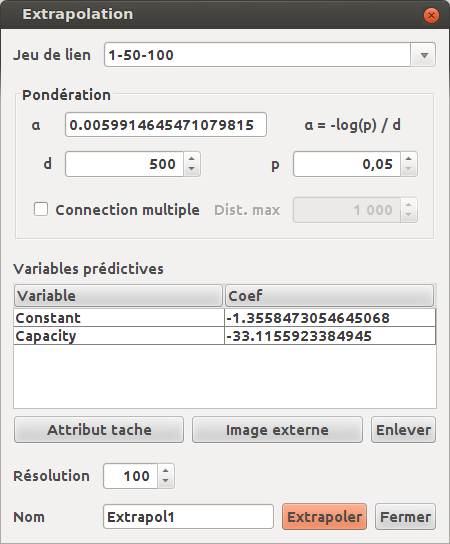
\includegraphics[scale=0.5]{img/manual-fr_img16.png} 
\end{figure}

Dans la nouvelle fenêtre qui s’affiche, l’utilisateur retrouve les paramètres du modèle tels qu’ils ont été décrits précédemment. La résolution de la grille (en mètres) indique le niveau de précision spatiale selon lequel cette extrapolation est effectuée. Ce critère a une forte incidence sur le temps de calcul nécessaire pour obtenir le résultat. Le résultat est archivé sous forme de couche raster au format *.tif et affiché dans la fenêtre principale.

\bigskip
Références : \cite{2012_SDM, 2012_graphab_EMS, 2013_SDM, 2013_SDM_rainette}


\section{Affichage}

\subsection{Propriétés des graphes}

Les propriétés des graphes sont accessibles par un clic droit sur le nom du graphe. Deux modes de visualisation des graphes sont disponibles : 
\begin{itemize}
	\item La vue topologique~affiche une vue simplifiée du graphe où les nœuds sont représentés par des cercles et les liens par des lignes droites de centroïde à centroïde. 
	\item La vue réaliste~affiche les taches d’habitat selon leurs limites réelles et les liens sont représentés par les chemins de moindre coût entre deux taches.  
\end{itemize}

\begin{figure}[H]
	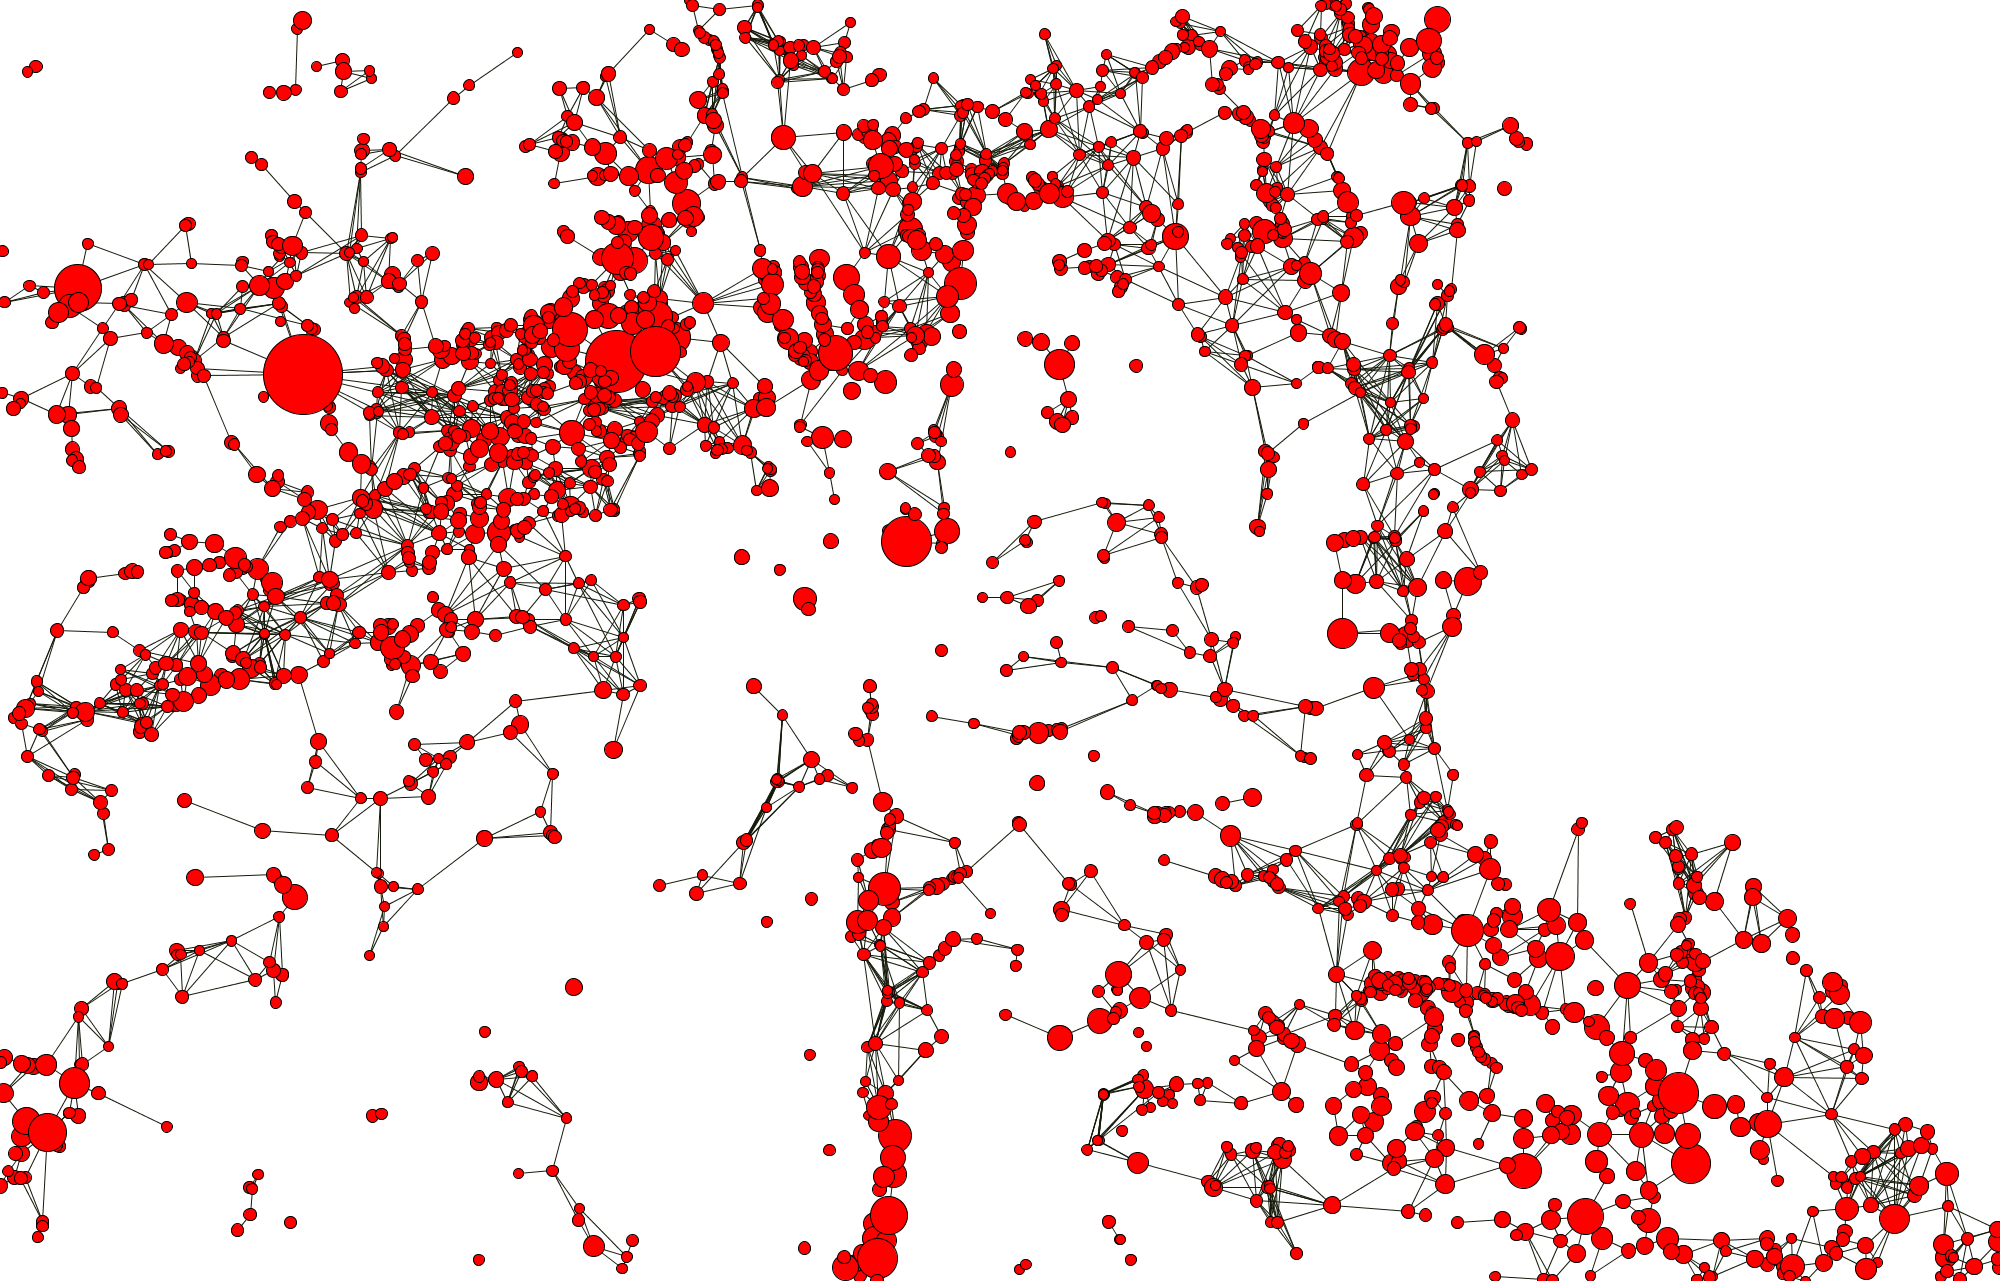
\includegraphics[scale=0.1]{img/manual-fr_img17.png} 
	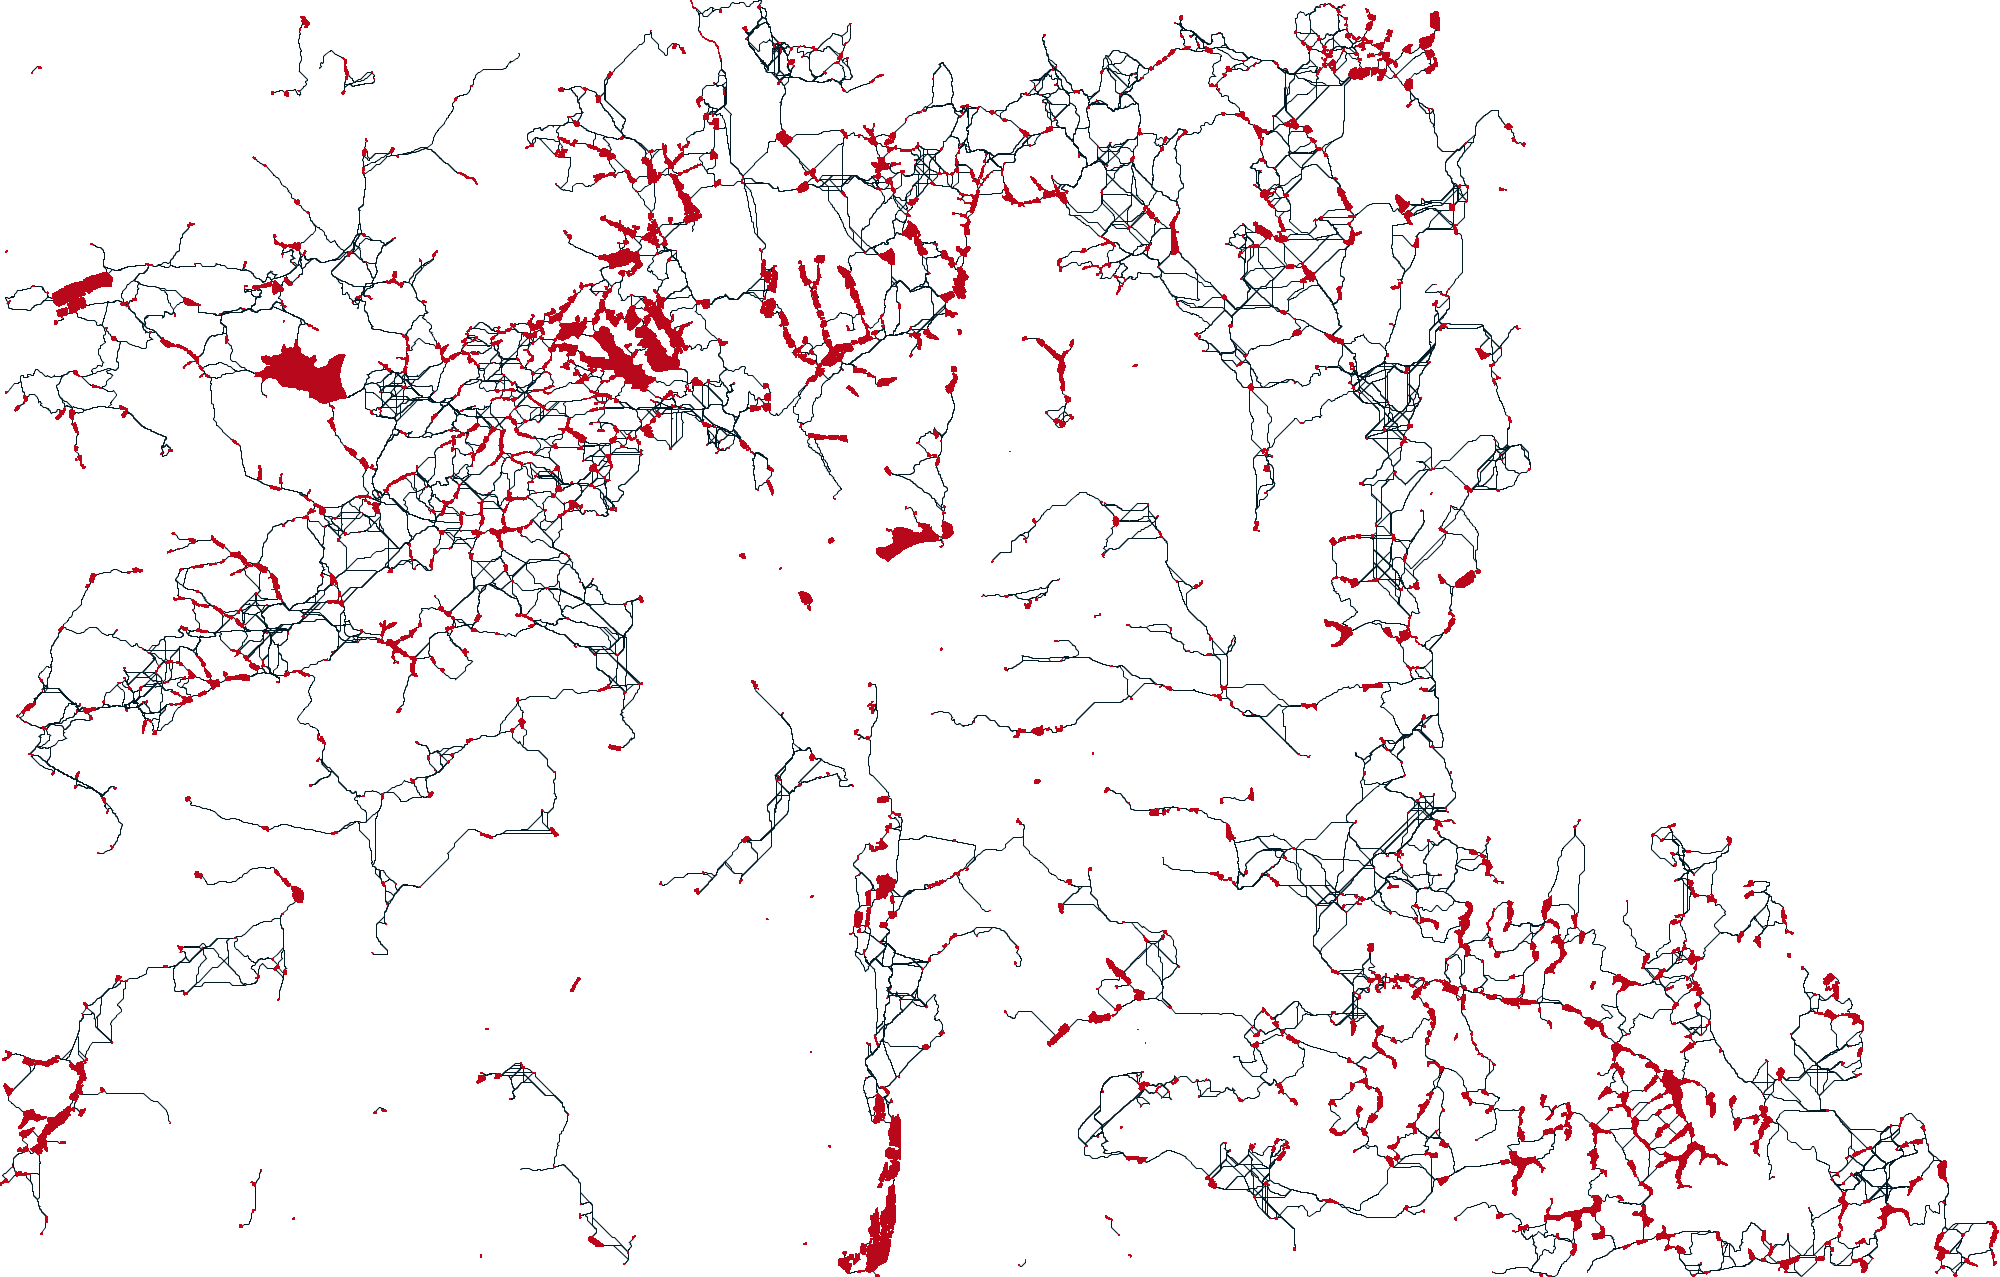
\includegraphics[scale=0.1]{img/manual-fr_img18.png} 
	\caption*{Gauche : vue topologique - Droite : vue réaliste}
\end{figure}


L'entrée Supprimer permet de supprimer le graphe sélectionné. Le projet est enregistré automatiquement après.

L'entrée Propriétés rappellent les paramètres utilisés pour la construction du graphe : le nom du graphe, le jeu de liens sélectionné, le type de graphe avec éventuellement le seuil de distance utilisé et le nombre de liens.

L'entrée Matrice OD (matrice Origine-Destination) permet de créer un tableau indiquant la distance entre chaque paire de nœuds pour le graphe sélectionné. L’unité de la distance dépend du type de distance utilisé pour ce graphe. L’absence de connexion entre deux nœuds est notée NaN (Not a Number). Cette  matrice est archivée dans le dossier du projet sous la forme d’un fichier texte nommé «~nom du graphe-odmatrix.txt~». 

\subsection{Propriétés des objets}
\label{properties}
Les propriétés de chaque jeu de liens, des éléments d’un graphe (nœuds, liens ou composantes) et des données ponctuelles sont accessibles par un clic droit sur chacun d’entre eux.

Le menu Style donne accès aux paramètres d’affichage des objets : couleur, épaisseur des contours, étiquettes, taille des symboles (pour les nœuds uniquement). Les objets peuvent être représentés de la même manière (symbole unique) ou en fonction d’un attribut. Il est possible d’appliquer une méthode de discrétisation pour classer les objets en fonction des valeurs de l’attribut sélectionné. Par défaut, la légende des objets est affichée dans la table des matières. Il est possible de la cacher en décochant le bouton Légende.

Le menu Export permet d’exporter les objets dans un fichier vecteur (*.shp) ou un fichier texte (*.txt).

Le menu Statistiques permet d’afficher la distribution des valeurs d’un ou plusieurs attributs : 
\begin{itemize}
	\item nuage de point : affiche un nuage de point mettant en relation les valeurs de deux attributs
	\item histogramme : affiche l’histogramme des valeurs d’un attribut.
\end{itemize}

Il est également possible d’afficher les valeurs d’un objet particulier en le sélectionnant à l’aide de la flèche. Après sélection, la valeur des attributs s’affiche dans une nouvelle colonne à droite. Il est possible de fermer cette colonne en cliquant sur le menu  Propriétés~ dans la barre du haut.

\begin{figure}[H]
	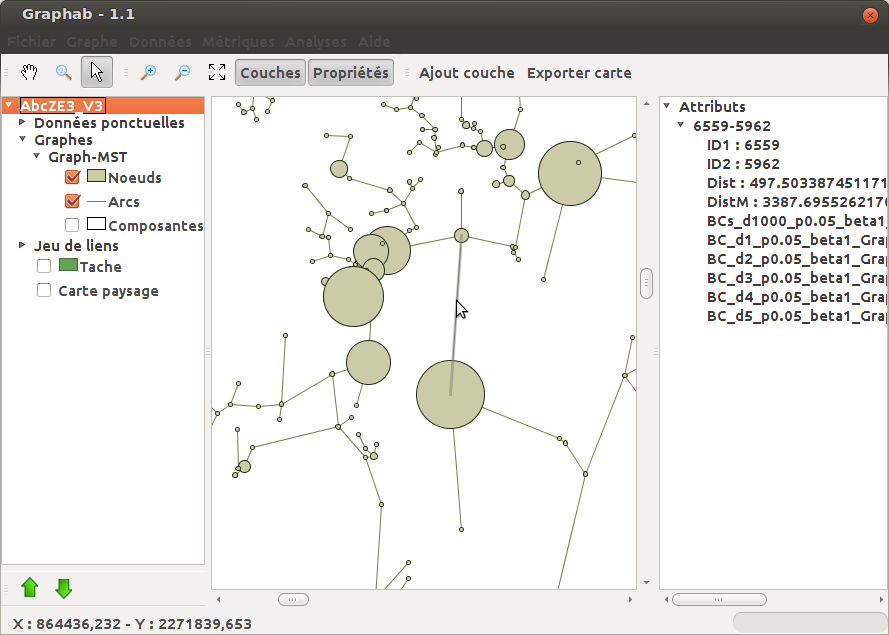
\includegraphics[scale=0.5]{img/manual-fr_img19.png} 
\end{figure}


\section{Capacités de traitement et limitations}
\label{limit}
Les méthodes basées sur les graphes sont connues pour fournir un cadre de modélisation efficace, mais peuvent poser une question de capacité de calcul. Deux points spécifiques ont reçu une attention particulière dans Graphab : (1) le calcul des jeux de liens, (2) le calcul des métriques de connectivité. Tous ces calculs ont été optimisés par parallélisation. Ce mode de développement améliore l'efficacité de calcul en utilisant une architecture multiprocesseur, un processeur quatre-cœur permettant théoriquement un calcul quatre fois plus rapide. 

Dans \cite{2012_graphab_EMS}, plusieurs tests ont été effectués afin de mesurer la capacité de calcul de Graphab dans différentes configurations. Trois configurations ont été comparées : 1) un cœur (3Go RAM) correspondant à un ordinateur standard ; 2) quatre cœurs (6 Go RAM) correspondant à une station de travail ; 3)  20 cœurs (15 Go RAM) correspondant à un serveur. La carte d’occupation du sol était un fichier raster de 14000*18000 pixels (252 millions de pixels) représentant l’occupation du sol de la région Franche-Comté (France) à une résolution spatiale de 10 mètres. La carte contenait 22 634 taches d’habitats. Le tableau \ref{perf} donne quelques temps de calcul pour la création de liens.

\begin{table}[H]
\begin{tabular}{|m{3.049cm}|m{3.049cm}|m{3.494cm}|m{3.0509999cm}|m{2.603cm}|}
\hline
Topologie & Distance & Ordinateur standard & Station de travail & Serveur\\
\hline
\multirow{2}{*}{Complète}
 & Euclidienne & 1927s (32 min) & 516s (8 min) & 133s (2 min)\\
\hhline{~----}
 & Moindre coût & 19252s (5h 21 min) & 4301s (1h 11 min) & 1037s (17 min)\\
\hline
\multirow{2}{*}{Planaire}
 & Euclidienne & 43s & 12s & 2.6s\\
\hhline{~----}
 & Moindre coût & 1080s (18 min) & 295s (5 min) & 82s (1 min)\\
\hline
\end{tabular}
\caption{Temps de calcul (en seconde) pour la création de différents jeux de liens.}
\label{perf}
\end{table}


La mémoire allouée au programme joue aussi un rôle important. Si il n’y a pas assez de mémoire vive, le calcul sera plus lent voire même ne pourra pas aboutir (message OutOfMemoryError ou GC Overhead). Le menu Fichier / Préférences / Mémoire permet de régler la mémoire allouée pour Graphab. Si vous avez une version 32 bits de Java, Graphab sera limité à environ 2 Go (2000 Mo) de mémoire. Si votre ordinateur a plus que 2 Go de mémoire vive il est fortement conseillé d’installer une version 64 bits de Java pour utiliser la mémoire disponible au-delà des 2 Go.


\section{Annexes}

\subsection{Détail de calcul des métriques}

Tableau récapitulatif des métriques présentes dans Graphab
\begin{table}[H]
	\begin{tabular}{|c|p{7cm}|l|c|c|c|c|}
		\hline
		\multirow{2}{*}{Famille} & \multirow{2}{*}{Métrique de connectivité} & \multirow{2}{*}{Code} & \multicolumn{3}{m{3cm}|}{\centering Niveau de calcul} & \multirow{2}{1.5cm}{Delta métriques}\\
		\hhline{~~~---~}
		&  &  & Global & Comp. & Local & \\
		\hline
		\multirow{6}{2cm}{Métriques pondérées}
		& Flux & F & × & × & × & \\
		& Probabilité de connectivité & PC & × & × &  & ×\\
		& Probabilité de connectivité flux & FPC &  &  & × & \\
		& Fractions de delta Probabilité de connectivité & dPC &  &  &  & ×\\
		& Indice de centralité intermédiaire & BC &  &  & × & \\
		& Indice intégral de connectivité & IIC & × & × &  & ×\\
		& Flux circuit & CF &  &  & × & \\
		\hline
		\multirow{4}{2cm}{Métriques de surface}
		& Taille moyenne des composantes & MSC & × &  &  & \\
		& Taille de la plus grande composante & SLC & × &  &  & \\
		& Probabilité de coïncidence de classe & CCP & × &  &  & \\
		& Taille de composante attendue & ECS & × &  &  & \\
		\hline
		\multirow{9}{2cm}{Métriques topologiques}
		& Degré & Dg &  &  & × & \\
		& Coefficient de groupement & CC &  &  & × & \\
		& Centralité de proximité & CCe &  &  & × & \\
		& Excentricité & Ec &  &  & × & \\
		& Corrélation de connectivité & CCor &  &  & × & \\
		& Elément de coupure & Cut &  &  & × & \\
		& Nombre de composantes & NC & × &  &  & \\
		& Diamètre & GD & × & × &  & ×\\
		& Indice d’Harary & H & × & × &  & ×\\
		\hline
	\end{tabular}

\end{table}

Termes mathématiques utilisés

\begin{table}[H]
\begin{tabular}{|m{3.24cm}|m{12.604cm}|}
\hline
Terme &
Signification\\\hline
$
n
$
 &
Nombre de taches\\\hline
$
\mathit{nc}
$
 &
Nombre de composantes\\\hline
$
{n}_{k}
$
 &
Nombre de taches de la composante k\\\hline
$
{N}_{i}
$
 &
Ensemble des taches voisines de la tache i\\\hline
$
{a}_{i}\text{~}
$
 &
Capacité de la tache i (en général sa surface)\\\hline
$
{\mathit{ac}}_{k}
$
 &
Capacité de la composante k (somme des capacités des taches qui la composent)\\\hline
$
A
$
 &
Surface de la zone d’étude\\\hline
$
{d}_{\mathit{ij}}\text{~}
$
 &
distance entre les taches i et j (en général la distance de moindre coût qui les sépare)\\\hline
$
{e}^{-\alpha {d}_{\mathit{ij}}}\text{~}
$
 &
Probabilité de déplacement entre les taches i et j\\\hline
$
\alpha 
$
 &
Frein de la distance vis-à-vis des déplacements\\\hline
$
\beta 
$
 &
Exposant permettant de pondérer plus ou moins la capacité\\\hline
\end{tabular}
\end{table}


\subsubsection{Métriques pondérées}

\begin{table}[H]
\begin{tabular}{|m{3.24cm}|m{4.4810004cm}m{7.924cm}|}

\hline
\multicolumn{3}{|m{16.044998cm}|}{Flux ($F$)}\\\hline
 &
\multicolumn{1}{m{4.4810004cm}|}{Formule} &
Signification\\\hline
Niveau~global &
\multicolumn{1}{m{4.4810004cm}|}{\begin{equation*}
F=\sum _{i=1}^{n}{\sum _{\begin{matrix}j=1\\j{\neq}i\end{matrix}}^{n}{{a}_{j}^{\beta }}}{e}^{-\alpha {d}_{\mathit{ij}}}
\end{equation*}
} &
Pour le graphe entier : somme des dispersions potentielles à partir de toutes les taches.\\\hline
Niveau~local &
\multicolumn{1}{m{4.4810004cm}|}{\begin{equation*}
{F}_{i}=\sum _{\begin{matrix}j=1\\j{\neq}i\end{matrix}}^{n}{{a}_{j}^{\beta }}{e}^{-\alpha {d}_{\mathit{ij}}}
\end{equation*}
} &
Pour la tache focale i : somme des capacités des taches différentes de i et pondérées en fonction de leur distance minimale à la tache focale en parcourant le graphe. Cette somme est un indicateur de la dispersion potentielle à partir de la tache i, ou inversement à destination de la tache i.

\\\hline
Valeurs &
\multicolumn{2}{m{12.6050005cm}|}{Les valeurs dépendent de la définition de a. Si a représente une surface, F exprime une surface.

Valeur minimale : 0

Valeur maximale : surface totale de l’habitat
}\\\hline
Commentaire &
\multicolumn{2}{m{12.6050005cm}|}{Le chemin du graphe utilisé est celui qui maximise  ${e}^{-\mathit{\alpha d}}$, c’est-à-dire celui qui minimise la distance d (ou le coût) entre les taches i et j.

Cette métrique est appelée Area Weigthed Flux (AWF) dans certaines références. Dans Graphab cependant, a est plus général car il représente la capacité des taches, qui peut être leur surface ou un autre critère choisi par l’utilisateur. De même la pondération est variable en fonction du paramètre $\beta $.

Dans CS22, AWF est calculé seulement à partir des taches reliées directement à la tache focale, alors que Graphab tient compte des taches indirectement connectées. 

}\\\hline
Références &
\multicolumn{2}{m{12.6050005cm}|}{
	\cite{Urban2001} \cite{Saura2009} \cite{2012_SDM}
}\\\hline
\end{tabular}
\end{table}


\begin{table}[H]
\begin{tabular}{|m{3.24cm}|m{4.4810004cm}m{7.924cm}|}

\hline
\multicolumn{3}{|m{16.044998cm}|}{Probabilité de Connectivité ($PC$)}\\\hline
 &
\multicolumn{1}{m{4.4810004cm}|}{Formule} &
Signification\\\hline
Niveau~global

Niveau composante

Delta &
\multicolumn{1}{m{4.4810004cm}|}{\begin{equation*}
\mathit{PC}=\frac{1}{{A}^{2}}\sum _{i=1}^{n}{\sum _{j=1}^{n}{{a}_{i}^{\beta }}}{{a}_{j}^{\beta }e}^{-\alpha {d}_{\mathit{ij}}}
\end{equation*}
} &
Pour le graphe entier : somme des produits de la capacité de tous les couples de taches pondérées par leur probabilité d’interaction, divisée par le carré de la zone d’étude. Ce rapport équivaut à la probabilité que deux individus tirés au hasard dans la zone d’étude parviennent à entrer en contact.

\\\hline
Valeurs &
\multicolumn{2}{m{12.6050005cm}|}{Les valeurs correspondant à une probabilité.

Valeur minimale : 0

Valeur maximale : 1
}\\\hline
Commentaire &
\multicolumn{2}{m{12.6050005cm}|}{Pour chaque couple de taches, le chemin du graphe utilisé est celui qui maximise  ${e}^{-\mathit{\alpha d}}$, c’est-à-dire celui qui minimise la distance d (ou le coût) entre les taches i et j.

Dans CS22, la pondération des capacités est fixée à 1 ; dans Graphab elle peut être modifiée.

Si a ne représente pas la surface des taches, le résultat n’est plus une probabilité.

}\\\hline
Référence &
\multicolumn{2}{m{12.6050005cm}|}{\cite{Saura2007}}\\\hline
\end{tabular}
\end{table}


\begin{table}[H]
\begin{tabular}{|m{3.24cm}|m{4.4810004cm}m{7.924cm}|}

\hline
\multicolumn{3}{|m{16.044998cm}|}{Probabilité de Connectivité Flux ($FPC$)}\\\hline
 &
\multicolumn{1}{m{4.4810004cm}|}{Formule} &
Signification\\\hline
Niveau~local &
\multicolumn{1}{m{4.4810004cm}|}{\begin{equation*}
{\mathit{FPC}}_{i}=\frac{1}{{A}^{2}}\sum _{j=1}^{n}{{{a}_{i}^{\beta }{a}_{j}^{\beta }e}^{-\alpha {d}_{\mathit{ij}}}}
\end{equation*}
} &
Somme des produits de la capacité de la tache focale avec toutes les autres taches, pondérées par leur probabilité d’interaction, divisée par le carré de la surface de la zone d’étude.

\\\hline
Valeurs &
\multicolumn{2}{m{12.6050005cm}|}{Valeur minimale : 0

Valeur maximale : 1
}\\\hline
Commentaire &
\multicolumn{2}{m{12.6050005cm}|}{Pour chaque couple de taches, le chemin du graphe utilisé est celui qui maximise  ${e}^{-\mathit{\alpha d}}$, c’est-à-dire celui qui minimise la distance d (ou le coût) entre les taches i et j.

Cette métrique est simplement la contribution locale d’une tache à l’indice $PC$, puisque~ $\mathit{PC}=\sum _{i}{{\mathit{FPC}}_{i}}$. Elle équivaut à  ${dPC}_{flux}+{dPC}_{area}$ non divisé par la valeur globale du $PC$. Cependant la métrique $FPC$ est obtenue plus rapidement car son calcul n’est pas fondé sur la suppression itérative des taches (mode delta).

}\\\hline
\end{tabular}
\end{table}


\begin{table}[H]
\begin{tabular}{|m{2.2cm}|m{5.5cm}m{7.924cm}|}

\hline
\multicolumn{3}{|m{16.044998cm}|}{Fractions de delta Probabilité de Connectivité ($dPC$, $dPC_{area}$, $dPC_{flux}$, $dPC_{connector}$)}\\\hline
 &
\multicolumn{1}{m{5.229cm}|}{Formules} &
Signification\\\hline
Delta &
\multicolumn{1}{m{5.229cm}|}{\begin{equation*}
{\mathit{dPC}}_{i}=\frac{(\mathit{PC}-{\mathit{PC}}_{i}^{'})}{\mathit{PC}}
\end{equation*}
\begin{equation*}
{{\mathit{dPC}}_{i}=\mathit{dPC}}_{\mathit{area}}+{\mathit{dPC}}_{\mathit{flux}}{+\mathit{dPC}}_{\mathit{connector}}
\end{equation*}
\begin{equation*}
{\mathit{dPC}}_{\mathit{area}}=\frac{{a}_{i}^{2\beta }}{{A}^{2}\mathit{PC}}
\end{equation*}
\begin{equation*}
{dPC}_{flux}=\frac{{FPC}_{i}}{PC}-{dPC}_{area}
\end{equation*}
} &
Taux de variation entre la valeur de l’indice PC et la valeur PC’ représentant la suppression de la tache i.

La valeur de $dPC$ se décompose en trois parties :

{}- $dPC_{area}$ correspond à la variation due à la perte de la surface suite à la suppression de la tache i ;

{}- $dPC_{flux}$ correspond à la variation due à la perte des interactions entre la tache i et les autres taches ;

{}- $dPC_{connector}$ correspond à la variation due à la modification des chemins reliant les autres taches et passant initialement par i.~\\\hline
Valeurs &
\multicolumn{2}{m{13.353cm}|}{Valeur minimale : 0

Valeur maximale : 1

}\\\hline
Commentaire &
\multicolumn{2}{m{13.353cm}|}{Dans CS22, la pondération des capacités est fixée à 1 ; dans Graphab elle peut être modifiée.

Si a ne représente pas la surface des taches, le résultat n’est plus une probabilité et $dPC_{area}$ n’exprime pas une perte de surface mais de capacité.

}\\\hline
Référence &
\multicolumn{2}{m{13.353cm}|}{\cite{Saura2010}}\\\hline
\end{tabular}
\end{table}


\begin{table}[H]
\begin{tabular}{|m{3.24cm}|m{4.4810004cm}m{7.924cm}|}
\hline
\multicolumn{3}{|m{16.044998cm}|}{Indice de centralité intermédiaire ($BC$)}\\\hline
 &
\multicolumn{1}{m{4.4810004cm}|}{Formule} &
Signification\\\hline
Niveau~local &
\multicolumn{1}{m{4.4810004cm}|}{\begin{equation*}
{\mathit{BC}}_{i}=\sum _{j}{\sum _{k}{{a}_{j}^{\beta }}}{a}_{k}^{\beta }{e}^{-\alpha {d}_{\mathit{jk}}}
\end{equation*}
\begin{equation*}
j,k{\in}\left\{1..n\right\},k<j,i{\in}{P}_{\mathit{jk}}
\end{equation*}
} &
Somme des plus courts chemins passant par la tache focale i, chaque chemin étant pondéré par le produit des capacités des taches reliées et de leur probabilité d’interaction.

Pjk représente l’ensemble des taches traversées par le plus court chemin entre les taches j et k.

\\\hline
Valeurs &
\multicolumn{2}{m{12.6050005cm}|}{Les valeurs dépendent du paramétrage. Elles correspondent à un poids de transit potentiel.

Valeur minimale : 0

Valeur maximale : surface totale de l’habitat au carré.

}\\\hline
Commentaire &
\multicolumn{2}{m{12.6050005cm}|}{Avec un paramétrage de $\alpha=0$ et $\beta =0$ (pondération uniforme des chemins), on retrouve l’indice $BC$ tel qu’il est utilisé dans d’autres types de graphes.

Un paramétrage de $\alpha=0$ et $\beta=1$ donne aux chemins un poids égal au produit des capacités des taches qu’ils relient, quelle que soit leur distance.

Dans \cite{2012_graphab_EMS, 2012_SDM}, l’indice $BC_l$ a été proposé pour pondérer plus fortement les chemins supérieurs au critère choisi (distance de dispersion par exemple). Mais des tests ont ensuite montré que cet indice était très fortement corrélé au $BC$ pondéré avec $\alpha=0$.

Dans \cite{Bodin2010}, le  ${\mathit{BC}}_{\mathit{pc}}$ correspond au BC pondéré avec d égal à la distance de dispersion,   $\alpha $ tel que  ${e}^{-\mathit{\alpha d}}=0.05$ et  $\beta=1$.

}\\\hline
Références &
\multicolumn{2}{m{12.6050005cm}|}{
\cite{Bodin2010}
\cite{2012_graphab_EMS}

}\\\hline
\end{tabular}
\end{table}


\begin{table}[H]
\begin{tabular}{|m{3.24cm}|m{4.4810004cm}m{7.924cm}|}

\hline
\multicolumn{3}{|m{16.044998cm}|}{Indice Intégral de Connectivité ($IIC$)}\\\hline
 &
\multicolumn{1}{m{4.4810004cm}|}{Formule} &
Signification\\\hline
Niveau~global

Niveau composante

Delta &
\multicolumn{1}{m{4.4810004cm}|}{\begin{equation*}
\mathit{IIC}=\frac{1}{{A}^{2}}\sum _{i=1}^{n}{\sum _{j=1}^{n}{{\frac{{a}_{i}{a}_{j}}{{1+\mathit{nl}}_{\mathit{ij}}}}}}
\end{equation*}
} &
Pour le graphe entier : produit des capacités des taches divisé par le nombre de liens qui les sépare, la somme étant divisée par le carré de la surface de la zone d’étude. IIC est construit comme l’indice PC, mais en utilisant l’inverse d’une distance topologique plutôt qu’une fonction exponentielle négative de la distance basée sur l’impédance des liens.

\\\hline
Valeurs &
\multicolumn{2}{m{12.6050005cm}|}{Valeur minimale : 0

Valeur maximale : 1

}\\\hline
Référence &
\multicolumn{2}{m{12.6050005cm}|}{\cite{Pascual2006}}\\\hline
\end{tabular}
\end{table}

\begin{table}[H]
	\begin{tabular}{|m{3.24cm}|m{4.4810004cm}m{7.924cm}|}
		\hline
		\multicolumn{3}{|m{16.044998cm}|}{Flux circuit ($CF$)}\\\hline
		&
		\multicolumn{1}{m{4.4810004cm}|}{Formule} &
		Signification\\\hline
		Niveau~local &
		\multicolumn{1}{m{4.4810004cm}|}{
			\begin{equation*}
			CF_{i}=\sum_{j}^n{c_i^j}
			\end{equation*}
		} &
		Somme des courants traversant la tache focale $i$.
		
		$c_i^j$ représente le courant à travers la tache $i$ lorsque un courant est émis depuis toutes les taches vers la tache $j$ (la tache $j$ est reliée à la terre)
		
		\\\hline
		Valeurs &
		\multicolumn{2}{m{12.6050005cm}|}{			
			Valeur minimale : 0
			
			Valeur maximale : $(n-1)(n-2)$ si $\beta=0$
			
			$(n-2)\sum_i^{n-1} a_i$ si $\beta=1$
			
		}\\\hline
		Commentaire &
		\multicolumn{2}{m{12.6050005cm}|}{
			La métrique $CF$ utilise la théorie des circuits électriques. Chaque lien du graphe correspond à une résistance électrique, les sources de courants et la terre sont quant à elles attachées aux taches.
			
			Si $\beta=0$ chaque tache émet un courant unitaire, si $\beta=1$ chaque tache émet un courant égal à sa capacité.
			
			Cette métrique peut être vue comme un équivalent de la métrique BC (avec $\alpha=0$ et $\beta=0$) qui tient compte de l'ensemble des chemins possibles et non pas uniquement du chemin le plus court.
			
		}\\\hline
		Références &
		\multicolumn{2}{m{12.6050005cm}|}{		
			\cite{2015_collisions}
		}\\\hline
	\end{tabular}
\end{table}


\subsubsection{Métriques de surface}

\begin{table}[H]
\begin{tabular}{|m{3.24cm}|m{4.4810004cm}m{7.924cm}|}

\hline
\multicolumn{3}{|m{16.044998cm}|}{Taille moyenne des composantes (MSC)}\\\hline
 &
\multicolumn{1}{m{4.4810004cm}|}{Formule} &
Signification\\\hline
Niveau~global &
\multicolumn{1}{m{4.4810004cm}|}{\begin{equation*}
\mathit{MSC}=\frac{1}{\mathit{nc}}\sum _{k=1}^{\mathit{nc}}{{\mathit{ac}}_{k}}
\end{equation*}
} &
Pour le graphe entier : moyenne des capacités des composantes.

\\\hline
Valeurs &
\multicolumn{2}{m{12.6050005cm}|}{Valeur minimale : capacité minimale

Valeur maximale :  $\mathit{SLC}$

}\\\hline
\end{tabular}
\end{table}


\begin{table}[H]
\begin{tabular}{|m{3.24cm}|m{4.4810004cm}m{7.924cm}|}

\hline
\multicolumn{3}{|m{16.044998cm}|}{Taille de la plus grande composante (SLC)}\\\hline
 &
\multicolumn{1}{m{4.4810004cm}|}{Formule} &
Signification\\\hline
Niveau~global &
\multicolumn{1}{m{4.4810004cm}|}{\begin{equation*}
\mathit{SLC}=\mathit{max}\{{\mathit{ac}}_{k}\}
\end{equation*}
} &
Pour le graphe entier : plus grande capacité des composantes.

\\\hline
Valeurs &
\multicolumn{2}{m{12.6050005cm}|}{Valeur minimale : capacité minimale

Valeur maximale : capacité maximale

}\\\hline
\end{tabular}
\end{table}


\begin{table}[H]
\begin{tabular}{|m{3.24cm}|m{4.4810004cm}m{7.924cm}|}

\hline
\multicolumn{3}{|m{16.044998cm}|}{Probabilité de coïncidence de classe (CCP)}\\\hline
 &
\multicolumn{1}{m{4.4810004cm}|}{Formule} &
Signification\\\hline
Niveau~global &
\multicolumn{1}{m{4.4810004cm}|}{\begin{equation*}
\mathit{CCP}=\sum _{k=1}^{\mathit{nc}}{{\left(\frac{{\mathit{ac}}_{k}}{\sum _{l}{{\mathit{ac}}_{l}}}\right)}^{2}}
\end{equation*}
} &
Pour le graphe entier : probabilité que deux points choisis au hasard sur le graphe appartiennent à la même composante.

\\\hline
Valeurs &
\multicolumn{2}{m{12.6050005cm}|}{Valeur minimale : capacité minimale (autant de composantes que de taches et capacités uniformes)

Valeur maximale : somme des capacités (1 seule composante)

}\\\hline
Référence &
\multicolumn{2}{m{12.6050005cm}|}{\cite{Pascual2006}}\\\hline
\end{tabular}
\end{table}


\begin{table}[H]
\begin{tabular}{|m{3.24cm}|m{4.4810004cm}m{7.924cm}|}

\hline
\multicolumn{3}{|m{16.044998cm}|}{Taille de composante attendue (ECS)}\\\hline
 &
\multicolumn{1}{m{4.4810004cm}|}{Formule} &
Signification\\\hline
Niveau~global &
\multicolumn{1}{m{4.4810004cm}|}{\begin{equation*}
\mathit{ECS}=\frac{1}{\sum _{k}{{\mathit{ac}}_{k}}}\sum _{k=1}^{\mathit{nc}}{{{\mathit{ac}}_{k}^{2}}}
\end{equation*}
} &
Pour le graphe entier : ?

\\\hline
Valeurs &
\multicolumn{2}{m{12.6050005cm}|}{Valeur minimale : capacité minimale (autant de composantes que de taches et capacités uniformes)

Valeur maximale : somme des capacités (1 seule composante)

}\\\hline
Référence &
\multicolumn{2}{m{12.6050005cm}|}{\cite{OBrien2006}}\\\hline
\end{tabular}
\end{table}


\subsubsection{Métriques topologiques}

\begin{table}[H]
\begin{tabular}{|m{3.24cm}|m{4.4810004cm}m{7.924cm}|}

\hline
\multicolumn{3}{|m{16.044998cm}|}{Indice d’Harary (H)}\\\hline
 &
\multicolumn{1}{m{4.4810004cm}|}{Formule} &
Signification\\\hline
Niveau~global  Niveau composante &
\multicolumn{1}{m{4.4810004cm}|}{\begin{equation*}
H=\sum _{i=1}^{n}{\sum _{\begin{matrix}j=1\\j{\neq}i\end{matrix}}^{n}{\frac{1}{{\mathit{nl}}_{\mathit{ij}}}}}
\end{equation*}
} &
Somme de l’inverse du nombre de liens séparant tous les couples de taches.

\\\hline
Valeurs &
\multicolumn{2}{m{12.6050005cm}|}{Valeur minimale : capacité minimale (autant de composantes que de taches et capacités uniformes)

Valeur maximale : somme des capacités (1 seule composante)

}\\\hline
Commentaire &
\multicolumn{2}{m{12.6050005cm}|}{Pour les couples de taches non connectées par un chemin on a :   ${\mathit{nl}}_{\mathit{ij}}=+{\infty}$}\\\hline
Référence &
\multicolumn{2}{m{12.6050005cm}|}{\cite{Ricotta2000}}\\\hline
\end{tabular}
\end{table}


\begin{table}[H]
\begin{tabular}{|m{3.24cm}|m{4.4810004cm}m{7.924cm}|}

\hline
\multicolumn{3}{|m{16.044998cm}|}{Diamètre (GD)}\\\hline
 &
\multicolumn{1}{m{4.4810004cm}|}{Formule} &
Signification\\\hline
Niveau~global  Niveau composante

Delta &
\multicolumn{1}{m{4.4810004cm}|}{\begin{equation*}
\mathit{GD}=\underset{\mathit{ij}}{\mathit{max}}{d}_{\mathit{ij}}
\end{equation*}
\begin{equation*}
\mathit{GD}=\underset{i}{\mathit{max}}{\mathit{Ec}}_{i}
\end{equation*}
} &
Distance la plus grande entre deux taches du graphe\\\hline
Valeurs &
\multicolumn{2}{m{12.6050005cm}|}{Valeur minimale : 0

Valeur maximale :  $+{\infty}$

}\\\hline
Commentaire &
\multicolumn{2}{m{12.6050005cm}|}{Quand les nœuds i et j ne sont pas connexes  ${d}_{\mathit{ij}}=0$

Cette métrique est la version globale de la métrique  ${\mathit{Ec}}_{i}$

}\\\hline
\end{tabular}
\end{table}
\begin{table}[H]
\raggedright
\begin{tabular}{|m{3.24cm}|m{4.4810004cm}m{7.924cm}|}

\hline
\multicolumn{3}{|m{16.044998cm}|}{Nombre de composantes (NC)}\\\hline
 &
\multicolumn{1}{m{4.4810004cm}|}{Formule} &
Signification\\\hline
Niveau~global 

 &
\multicolumn{1}{m{4.4810004cm}|}{\begin{equation*}
\mathit{NC}=\mathit{nc}
\end{equation*}
} &
Nombre de composantes du graphe\\\hline
Valeurs &
\multicolumn{2}{m{12.6050005cm}|}{Valeur minimale : 1

Valeur maximale :  $n$

}\\\hline
\end{tabular}
\end{table}
\begin{table}[H]
\raggedright
\begin{tabular}{|m{3.24cm}|m{4.4810004cm}m{7.924cm}|}

\hline
\multicolumn{3}{|m{16.044998cm}|}{Degré du noeud (Dg)}\\\hline
 &
\multicolumn{1}{m{4.4810004cm}|}{Formule} &
Signification\\\hline
Niveau~local 

 &
\multicolumn{1}{m{4.4810004cm}|}{\begin{equation*}
{\mathit{Dg}}_{i}=\left|{N}_{i}\right|
\end{equation*}
} &
Nombre de taches voisines de la tache i\\\hline
Valeurs &
\multicolumn{2}{m{12.6050005cm}|}{Valeur minimale : 0

Valeur maximale :  $n$

}\\\hline
Commentaire &
\multicolumn{2}{m{12.6050005cm}|}{Il y a équivalence entre le degré d’un nœud et le nombre de nœuds voisins car les graphes ne sont pas orientés et ne contiennent pas de boucle.

}\\\hline
\end{tabular}
\end{table}
\begin{table}[H]
\raggedright
\begin{tabular}{|m{3.24cm}|m{5.303cm}m{7.103cm}|}

\hline
\multicolumn{3}{|m{16.046cm}|}{Coefficient de groupement (CC)}\\\hline
 &
\multicolumn{1}{m{5.303cm}|}{Formule} &
Signification\\\hline
Niveau~local 

 &
\multicolumn{1}{m{5.303cm}|}{\begin{equation*}
{\mathit{CC}}_{i}=\frac{1}{\left|{N}_{i}\right|\left(\left|{N}_{i}\right|-1\right)}\sum _{j{\in}{N}_{i}}{\left|{N}_{i}{\cap}{N}_{j}\right|}
\end{equation*}
} &
Rapport du nombre de nœuds voisins de i voisins entre eux sur le total possible.\\\hline
Valeurs &
\multicolumn{2}{m{12.606cm}|}{Valeur minimale : 0

Valeur maximale : 1}\\\hline
Commentaire &
\multicolumn{2}{m{12.606cm}|}{Si  $\left|{N}_{i}\right|{\leq}1\rightarrow {\mathit{CC}}_{i}=0$ }\\\hline
\end{tabular}
\end{table}
\begin{table}[H]
\raggedright
\begin{tabular}{|m{3.24cm}|m{4.4810004cm}m{7.924cm}|}

\hline
\multicolumn{3}{|m{16.044998cm}|}{Centralité de proximité (CCe)}\\\hline
 &
\multicolumn{1}{m{4.4810004cm}|}{Formule} &
Signification\\\hline
Niveau~local 

 &
\multicolumn{1}{m{4.4810004cm}|}{\begin{equation*}
{\mathit{CCe}}_{i}=\frac{1}{{n}_{k}-1}\sum _{\begin{matrix}j=1\\j{\neq}i\end{matrix}}^{{n}_{k}}{{d}_{\mathit{ij}}}
\end{equation*}
} &
Distance moyenne de la tache i vers toutes les autres taches de sa composante k. \\\hline
Valeurs &
\multicolumn{2}{m{12.6050005cm}|}{Valeur minimale : 0

Valeur maximale :  $+{\infty}$

}\\\hline
Commentaire &
\multicolumn{2}{m{12.6050005cm}|}{Si  ${n}_{k}=1\rightarrow {\mathit{CCe}}_{i}=0$ }\\\hline
\end{tabular}
\end{table}
\begin{table}[H]
\raggedright
\begin{tabular}{|m{3.24cm}|m{4.4810004cm}m{7.924cm}|}

\hline
\multicolumn{3}{|m{16.044998cm}|}{Excentricité (Ec)}\\\hline
 &
\multicolumn{1}{m{4.4810004cm}|}{Formule} &
Signification\\\hline
Niveau~local 

 &
\multicolumn{1}{m{4.4810004cm}|}{\begin{equation*}
{\mathit{Ec}}_{i}=\underset{j}{\mathit{max}}{d}_{\mathit{ij}}
\end{equation*}
} &
Distance maximale de la tache i vers une autre tache de sa composante. \\\hline
Valeurs &
\multicolumn{2}{m{12.6050005cm}|}{Valeur minimale : 0

Valeur maximale :  $+{\infty}$

}\\\hline
\end{tabular}
\end{table}
\begin{table}[H]
\raggedright
\begin{tabular}{|m{3.24cm}|m{4.4810004cm}m{7.924cm}|}

\hline
\multicolumn{3}{|m{16.044998cm}|}{Corrélation de connectivité (CCor)}\\\hline
 &
\multicolumn{1}{m{4.4810004cm}|}{Formule} &
Signification\\\hline
Niveau~local 

 &
\multicolumn{1}{m{4.4810004cm}|}{\begin{equation*}
{\mathit{CCor}}_{i}=\frac{{\left|{N}_{i}\right|}^{2}}{\sum _{j{\in}{N}_{i}}{\left|{N}_{j}\right|}}
\end{equation*}
} &
Rapport entre le degré du nœud i et le degré de ses nœuds voisins j\\\hline
Valeurs &
\multicolumn{2}{m{12.6050005cm}|}{Valeur minimale : 0

Valeur maximale :  $\left|{N}_{i}\right|$}\\\hline
Commentaire &
\multicolumn{2}{m{12.6050005cm}|}{Si  $\left|{N}_{i}\right|=0\rightarrow {\mathit{CCor}}_{i}=0$}\\\hline
Référence &
\multicolumn{2}{m{12.6050005cm}|}{\cite{Minor2008}}\\\hline
\end{tabular}
\end{table}

\pagebreak

\bibliographystyle{graphab}
\bibliography{graphab}


\end{document}
